\section{Efficiencies}
\label{sec:eff}

The lack of simulated samples at every conceivable point in the $(m_\db, \tau_\db$) plane means
that the points that are available must be used to interpolate (and extrapolate) to all regions.
Assuming that the efficiencies vary continuously, it is possible to parameterize efficiencies using
spline interpolation.
This is done by pararameterizing the way that efficiency varies with mass and lifetime.

The efficiency due to the \lhcb acceptance region is stable as a function of mass, but does vary
slightly with mass, from \approx$18\pc$ for a $\mass{\db}=214\mev$ sample, to \approx$15\pc$ for a
$\mass{\db}=4000\mev$ sample.


\subsection{Reconstruction and stripping}
The reconstruction and stripping efficiencies are obtained from simulation and given in
\Tab{tab:eff:summary}.
Samples generated with larger lifetime have lower efficiencies because the Dark
Bosons will increasingly decay outside of the \velo.
This is also the case for low $m(\db)$, where there is a larger boost.
The evolution of the total efficiency as a function of mass (for the $100\ps$ samples) is shown in
\Fig{fig:eff:spline}.



%%mass |  tau |      reco |   trigger |    sel   |    BDT   |    TOTAL
%%2500 |   10 |     10.13 |     75.45 |    70.46 |    84.27 |     4.54
%%2500 |  100 |      3.21 |     67.61 |    70.58 |    83.79 |     1.28
%%2500 | 1000 |      0.40 |     64.38 |    70.53 |    85.26 |     0.15



\begin{figure}
  \begin{center}
    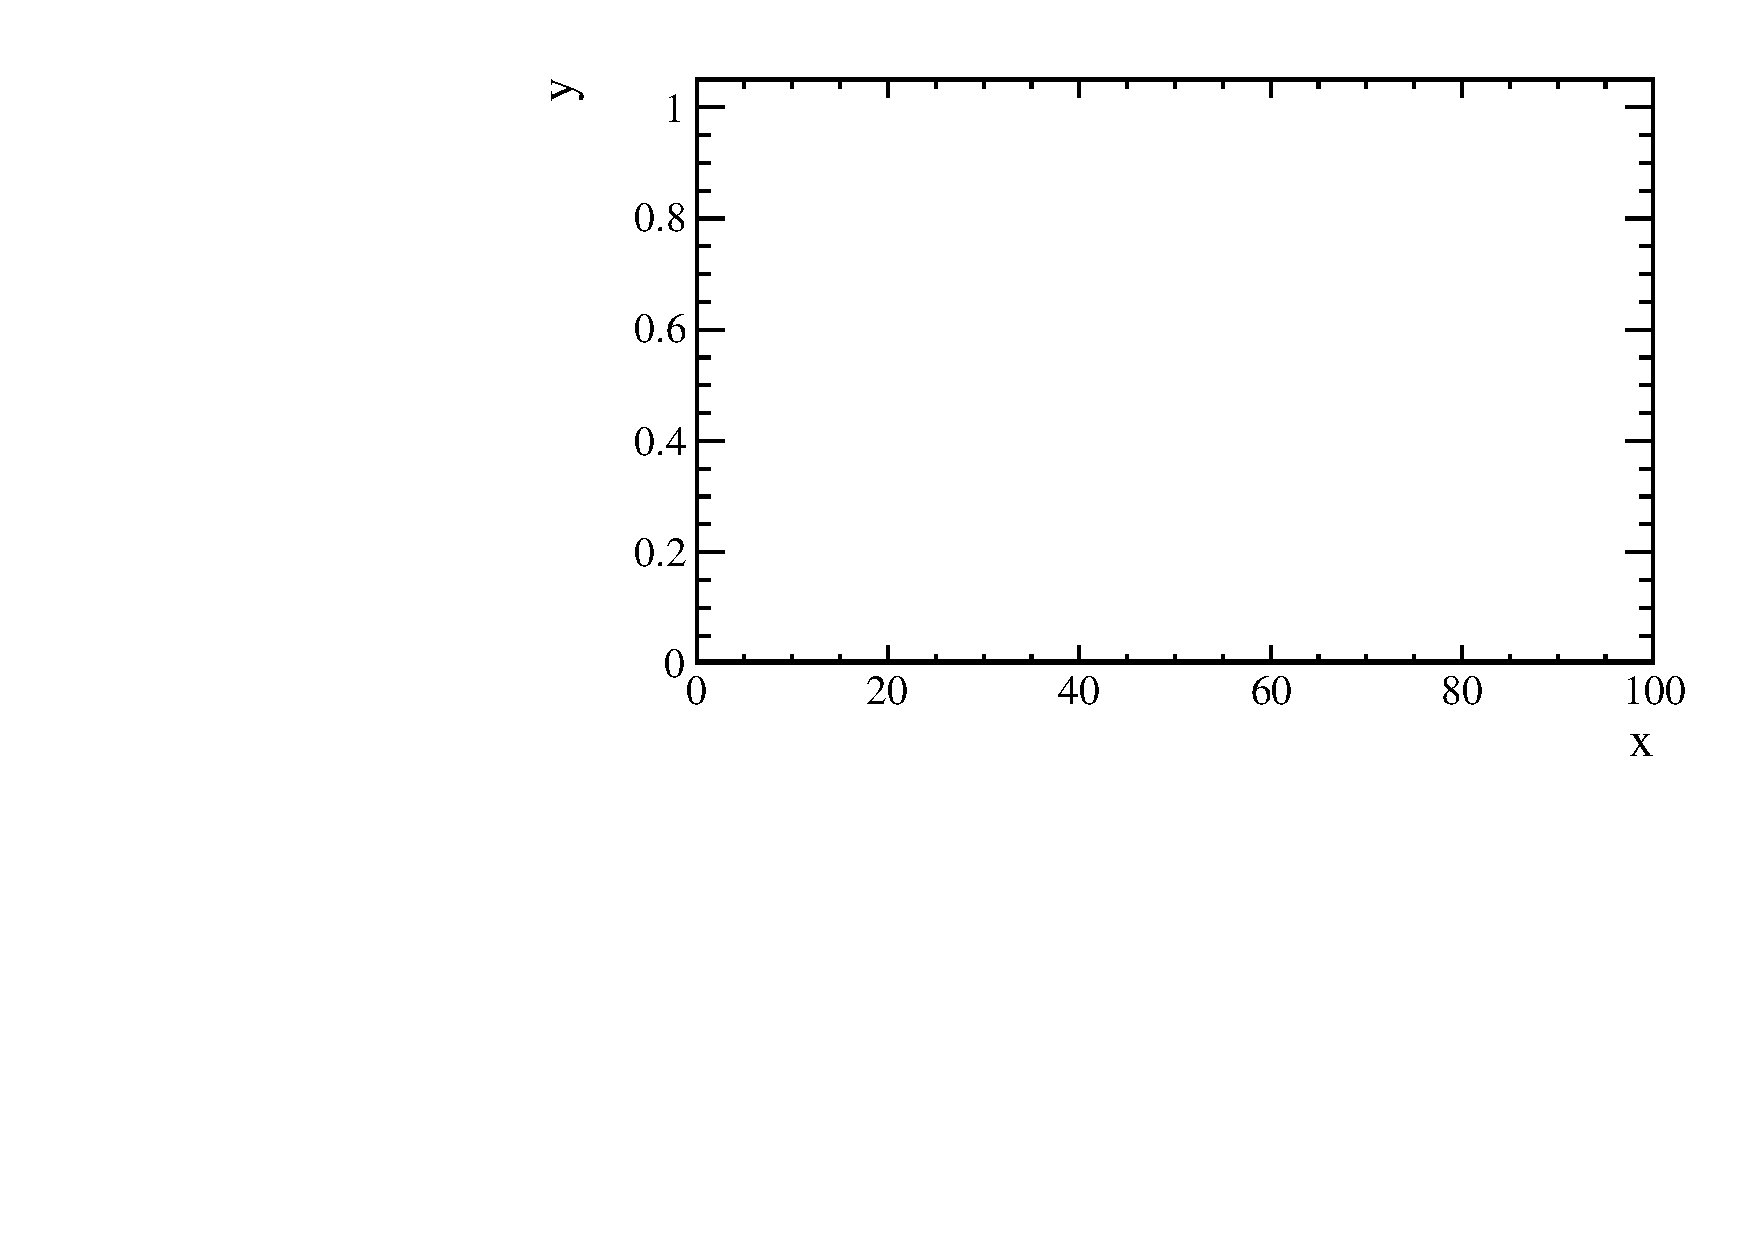
\includegraphics[width=0.48\textwidth]{blank}
    \caption{
      Evolution of the total efficiency for a \db with $\lifetime{\db}=100\ps$, where
      black points indicate the sampled masses, and the red line is the interpolated cubic spline
      intersecting each point.
    }
    \label{fig:eff:spline}
  \end{center}
\end{figure}

%\subsection{Normalization channel}
%The normalization channel is restricted in \qsq region, between 1.1 and $6.0\gevgev$.
%Using generator level simulation, it is determined that $(20.11\pm0.06)\%$ of generated events lie
%in this region.





\subsection{Lifetime resolution}
The lifetime resolution is obtained by fitting
$\Delta\tau=\tau^\mathrm{meas}_{\db}-\tau^\mathrm{true}_{\db}$, as shown in
\Fig{fig:taures:zoom}, and finding the $3\sigma$ limits of these
probability density functions.
For $m_{\mu\mu} > 250\mev$ the $\tau$ measurement is unbiased and has nearly uniform resolution.
However, for dimuon masses close to threshold, where the break up momentum is small, the lifetime
measurement is biased and less precise.
There is a strong difference between the resolution in the  214 and the 250\mev samples.
For this reason, small samples of simulated signal events were produced at 220 and 235\mev to aid
with the understanding of the detector response in this dimuon mass region.

\begin{figure}
  \begin{center}
    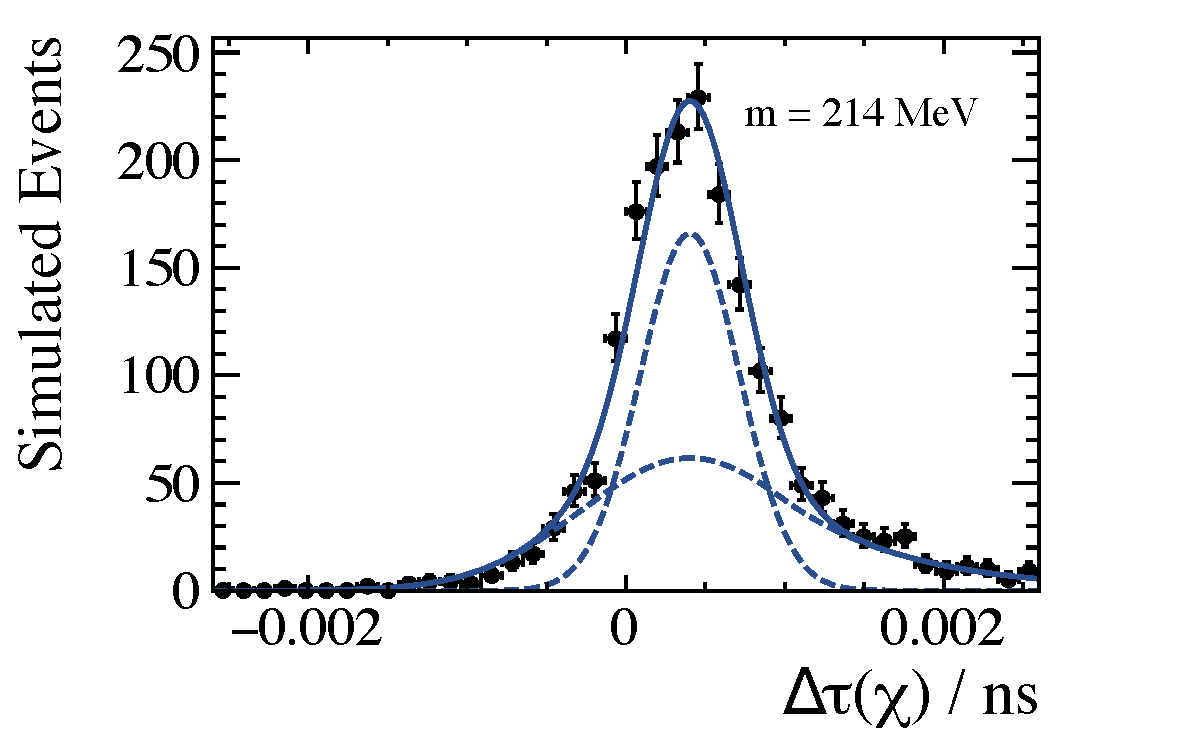
\includegraphics[width=0.42\textwidth]{anaTauResZoom_214}
    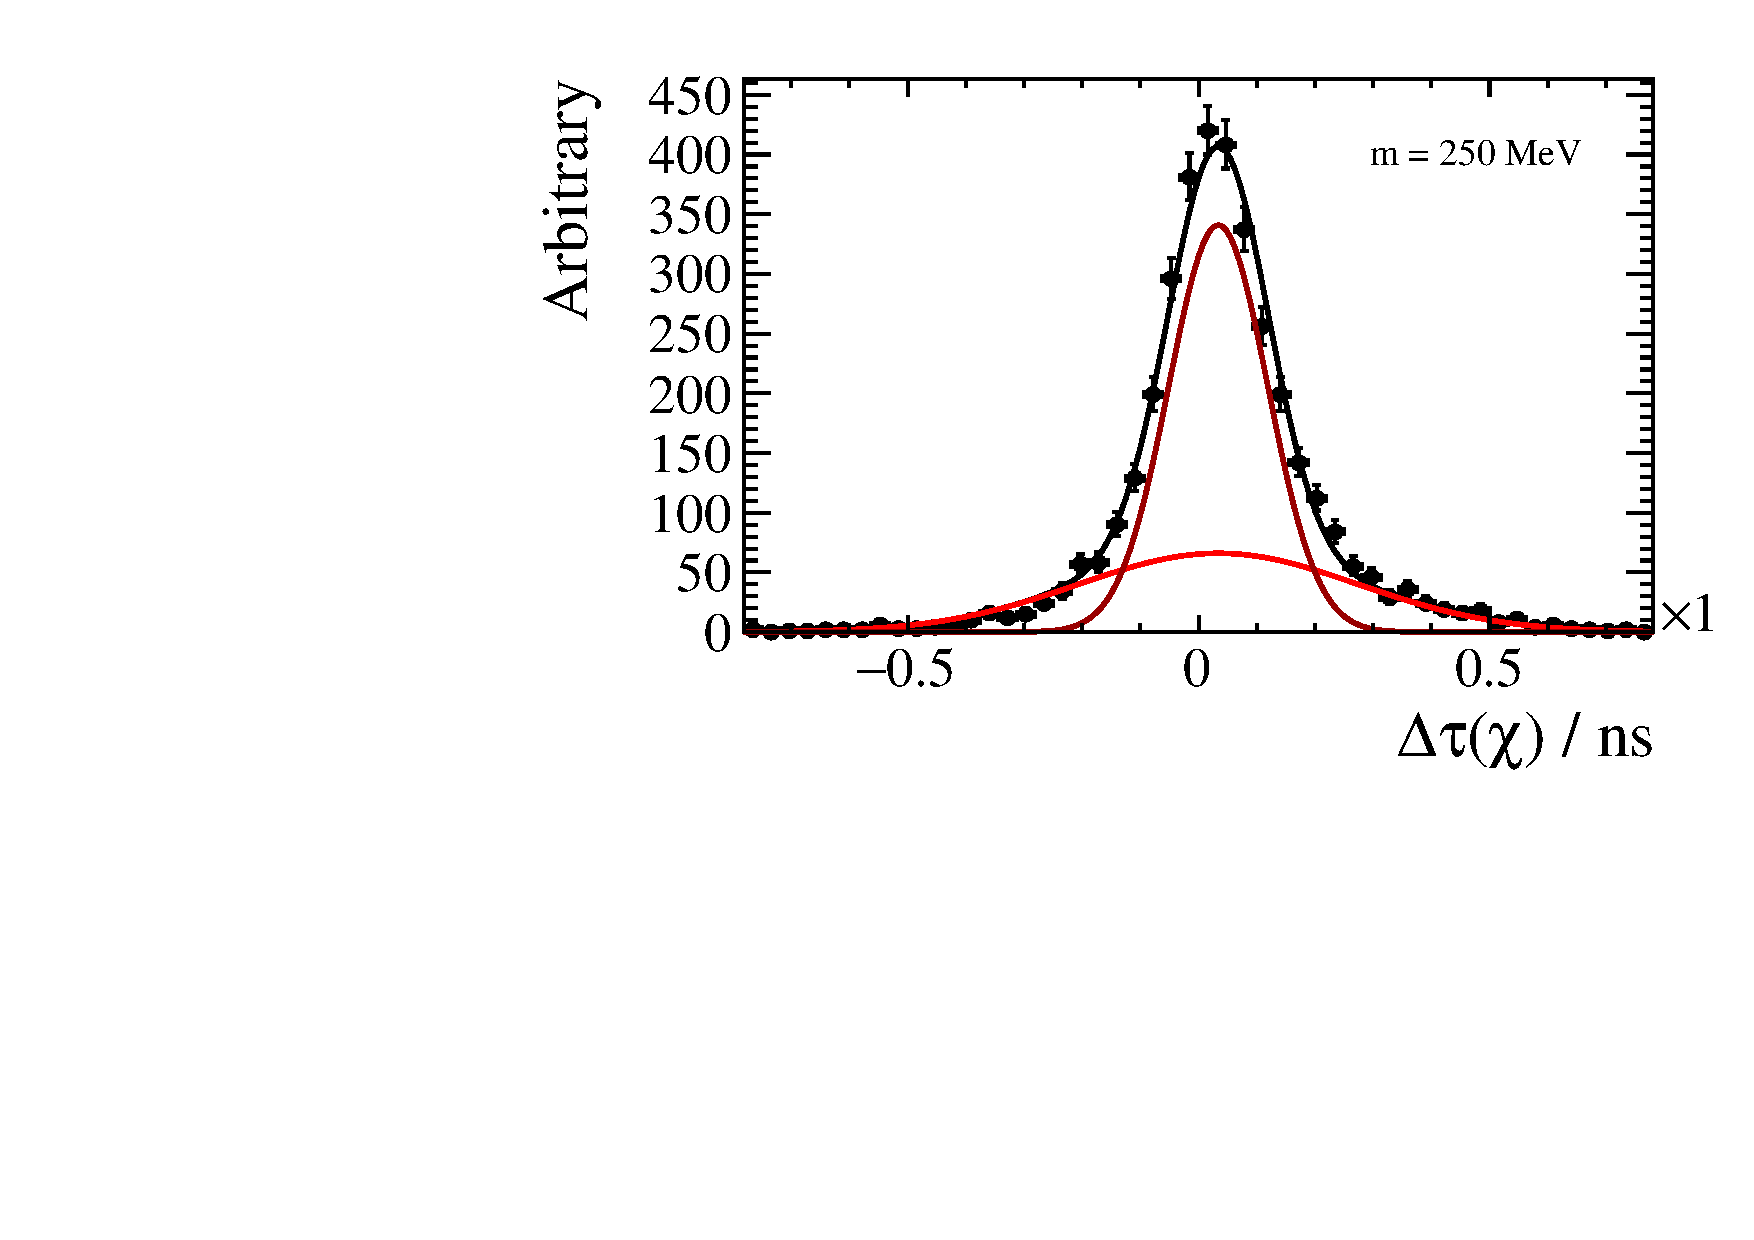
\includegraphics[width=0.42\textwidth]{anaTauResZoom_250}
    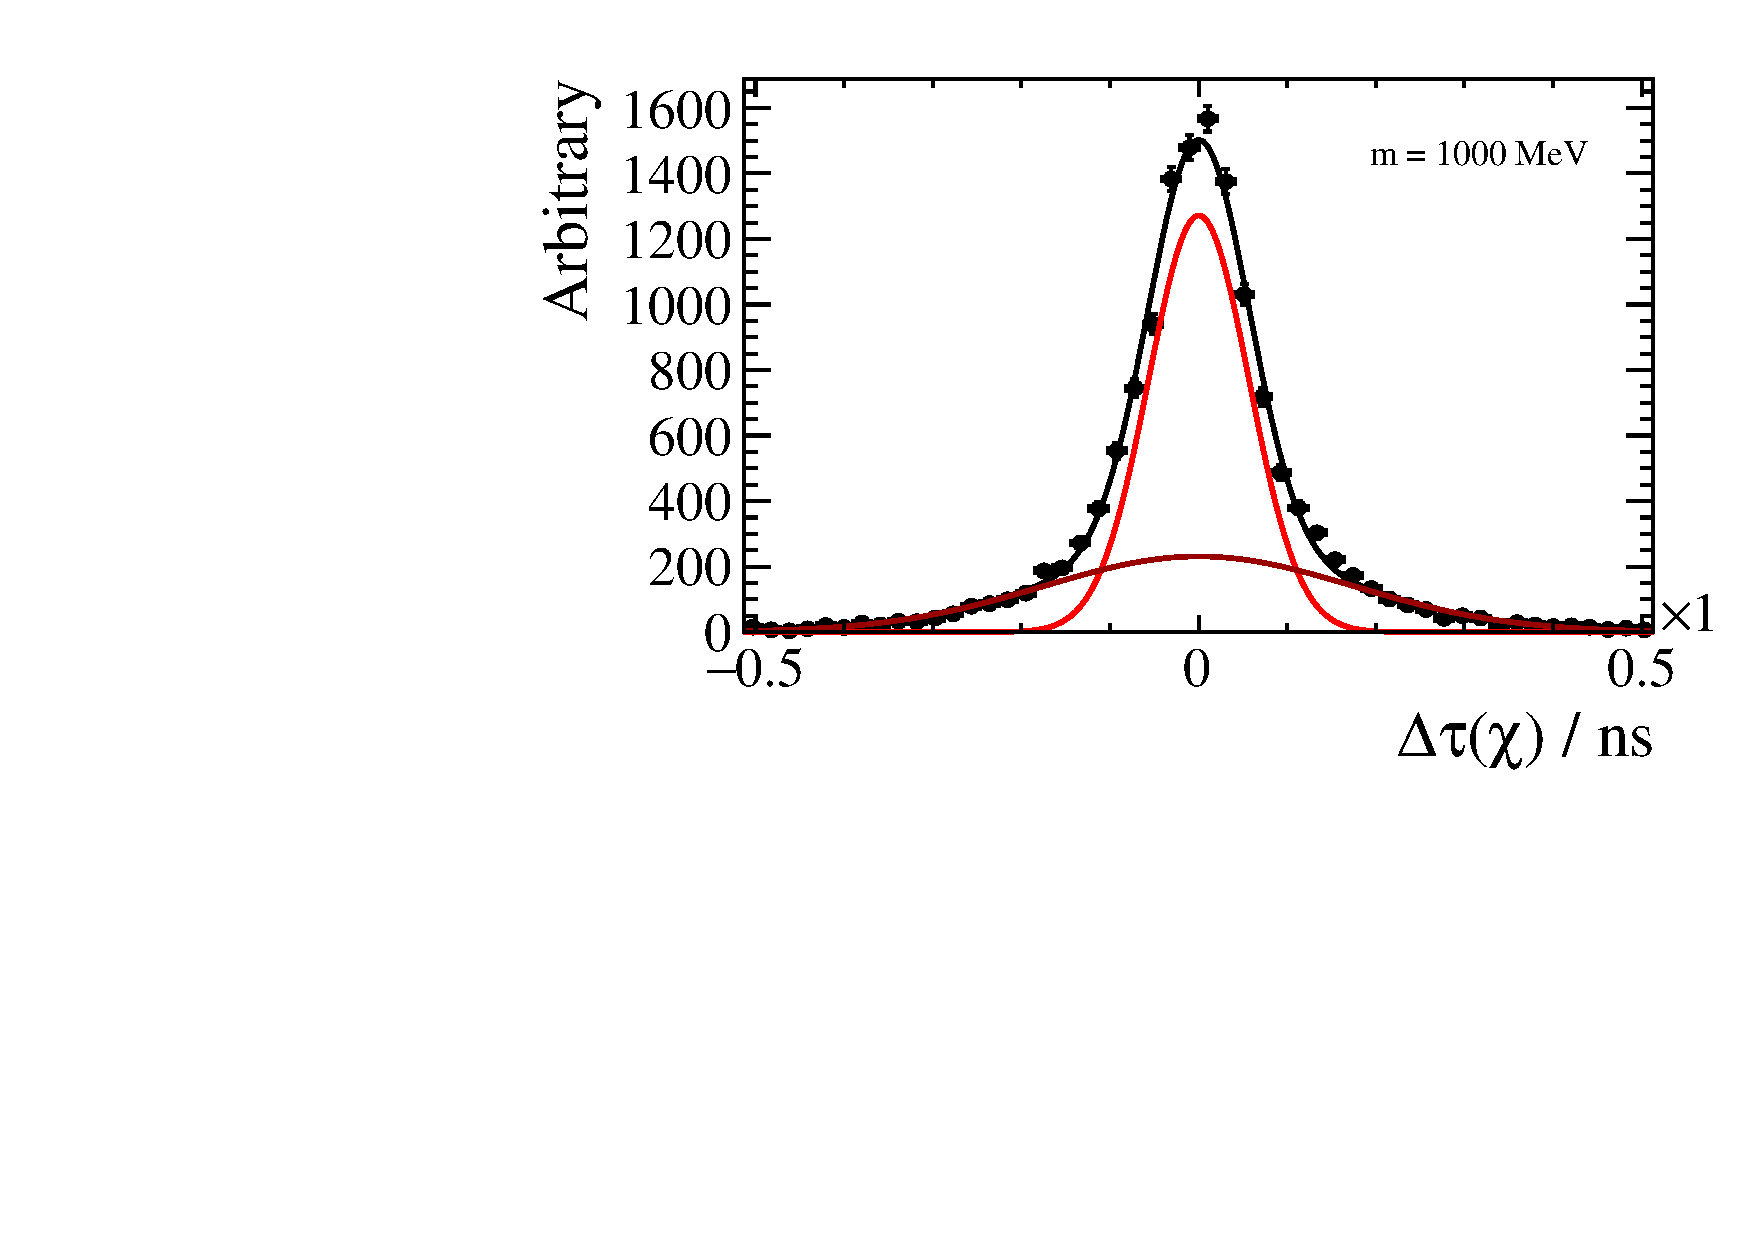
\includegraphics[width=0.42\textwidth]{anaTauResZoom_1000}
    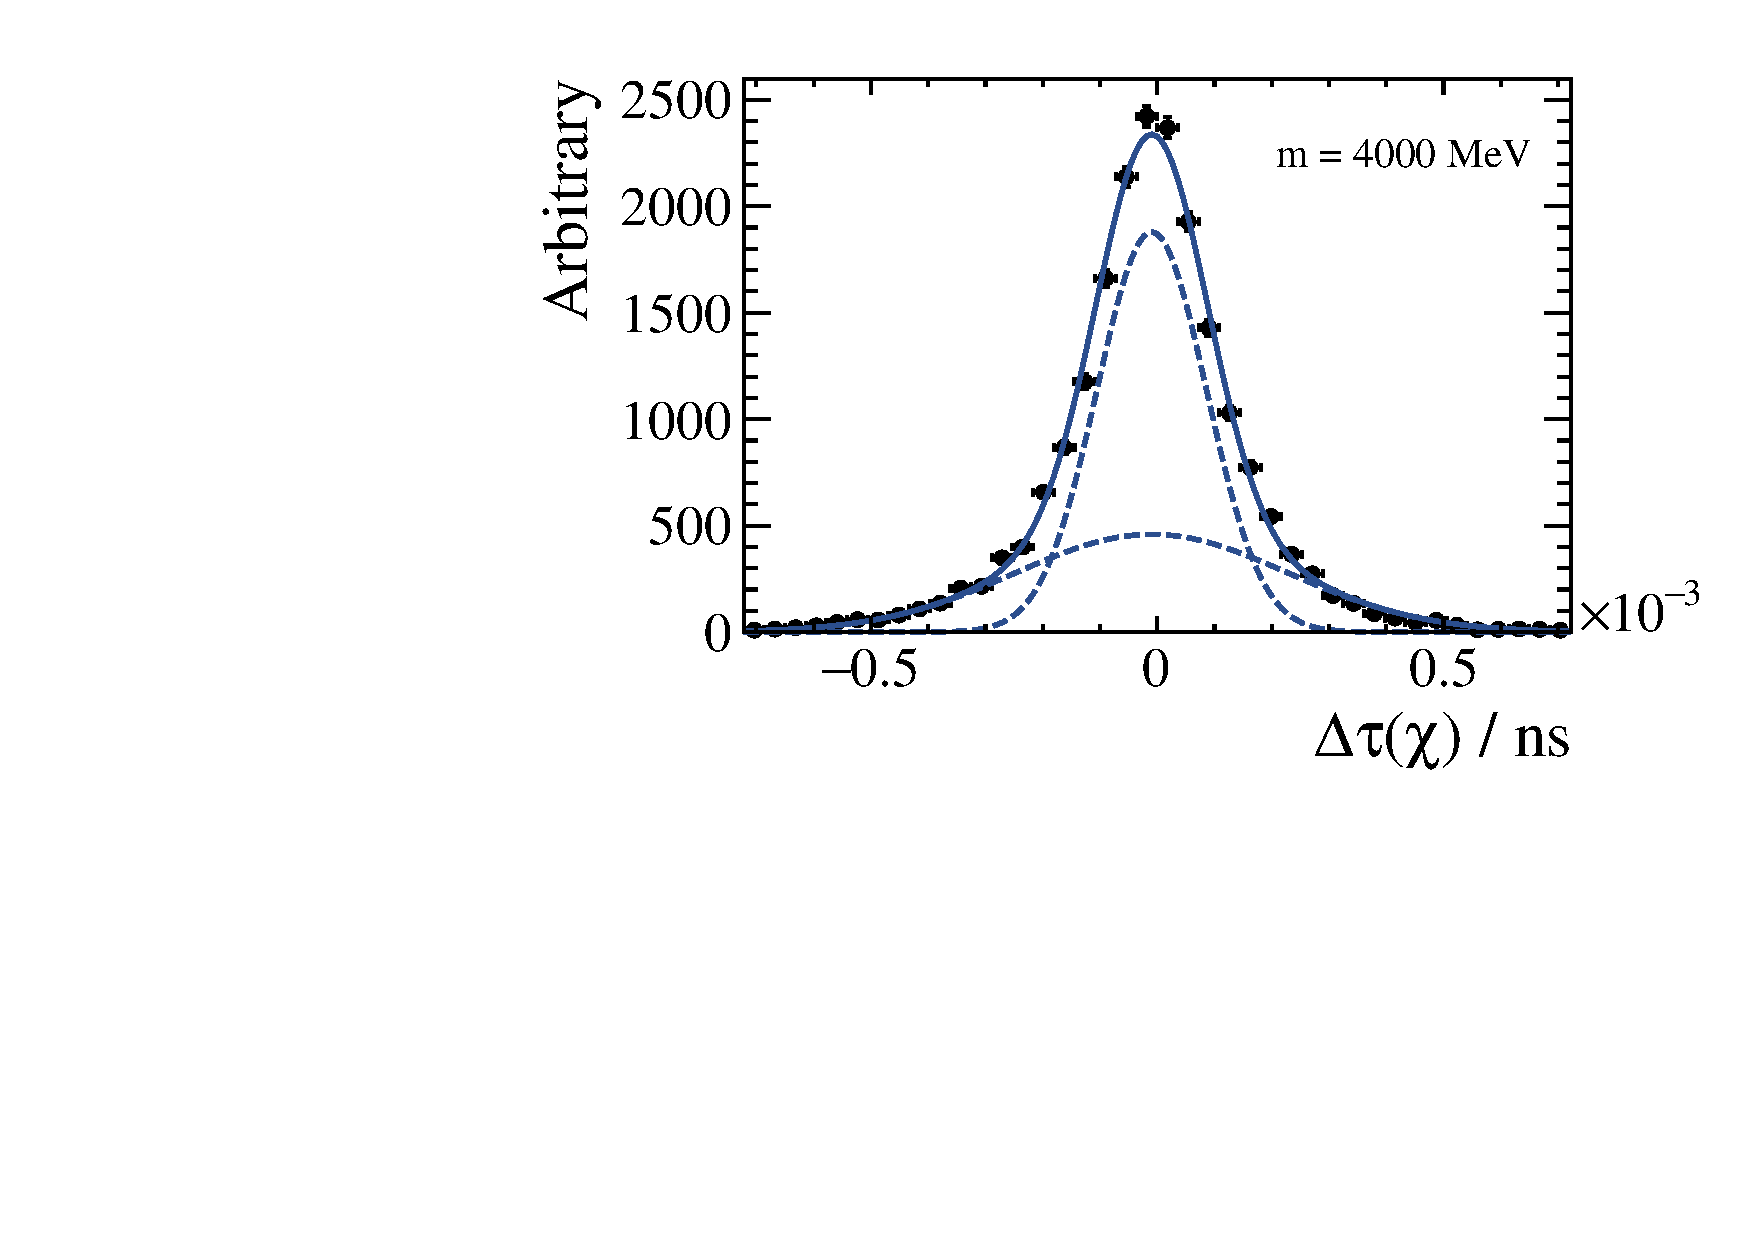
\includegraphics[width=0.42\textwidth]{anaTauResZoom_4000}
  \end{center}
  \caption{
    Fits to the lifetime resolution parameter, $\Delta\tau$, for individual mass samples.
    Each fit for $m\geq250\mev$ is made using a double Gaussian function, and for $m<250\mev$ the
    wider Gaussian has an exponential tail on the right-hand side.
  }
  \label{fig:taures:zoom}
\end{figure}

The source of the poor mass resolution at low mass is the \mumu opening angle, which is small near
the dimuon mass threshold.
This results in the separation of the hits in the first \velo station of the $\mu^+$ and $\mu^-$
being comparable to the resolution of the \velo strips which results in poor spatial resolution on
the SV position.
Furthermore, the hits are often merged in the \velo, producing a reconstructed SV position
downstream of the true position.
From the distributions of reconstructed and generated opening angles for $m=214\mev$ in
Fig.~\ref{fig:opening:gen},
it can be seen that there is no bias once the \mumu opening angle exceeds $\sim0.002$ radians.
Vetoing all events below this threshold is a very inefficient solution at low dimuon
masses, (see Fig.~\ref{fig:opening:gen}).
Instead, the bias is accounted for, as described below.

\begin{figure}
  \begin{center}
    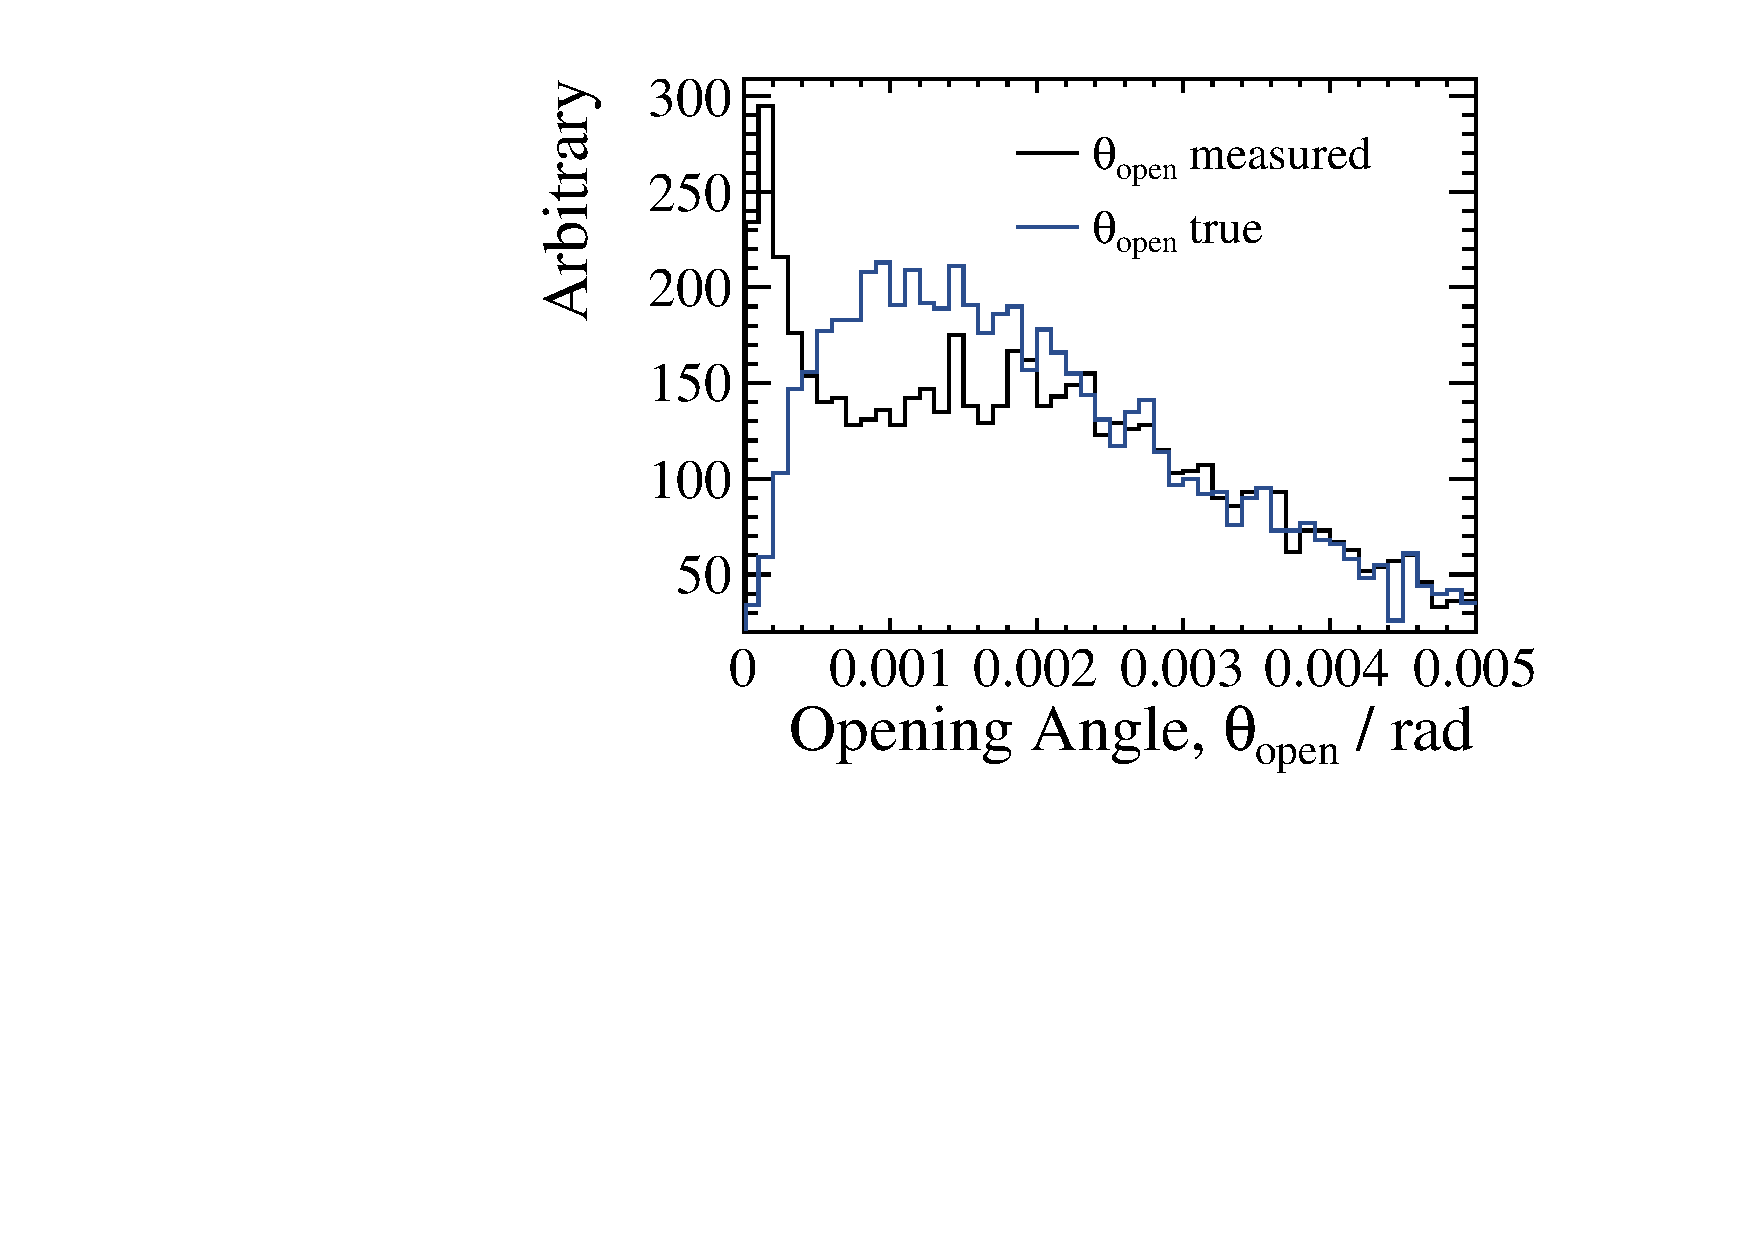
\includegraphics[width=0.48\textwidth]{ana214Opening}
    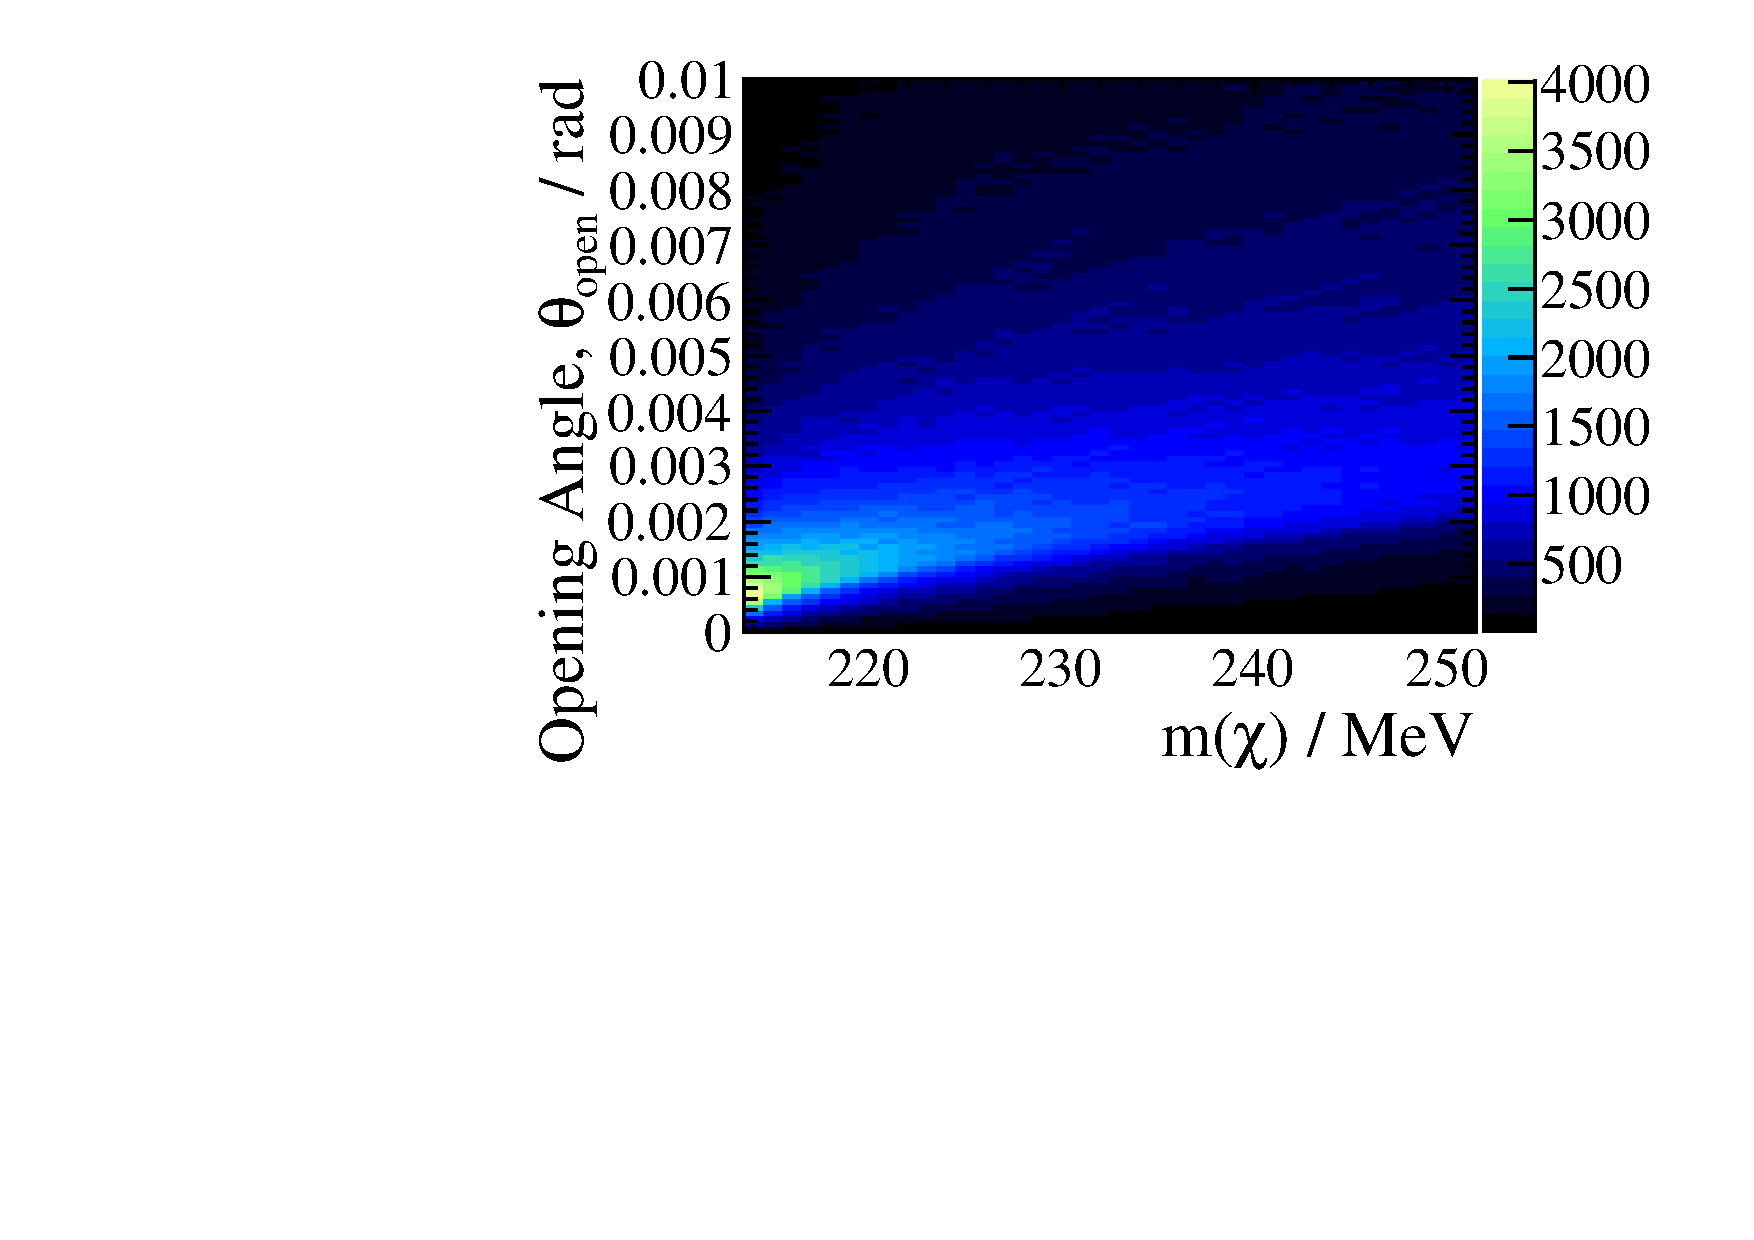
\includegraphics[width=0.48\textwidth]{anaGenLevelOpening}
  \end{center}
  \caption{\small
    The opening angle of the two muons decaying from the \db is highly dependent on \mdb; for low
    dimuon masses the opening angle measurement is biased.
    For $\mdb=214\mev$ the difference between generated and reconstructed opening angles are shown,
    (left) the greatest difference being below $\theta_\mathrm{open}=0.002$.
    Generator level distributions of opening angles for a range of masses,
    (right) show that most \db decays have $\theta_\mathrm{open}>0.002$ for
    $\mdb\gtrsim235\mev$.
  }
  \label{fig:opening:gen}
\end{figure}

The observation of the discrepancy between real and true opening angle can be verified using data
from a decay channel with very high statistics, for example,
the decay \decay{\Bd}{\kpi\mumu}, where the muons can come from any resonance.
Figure~\ref{fig:oa:2d} shows how the opening angle of the \kpi system changes with its invariant
mass (for $m_{\kpi}<900\mev$); it is seen that at threshold, the opening angle is observed to be
very small for low masses, especially at threshold, $m_{\Kp} + m_{\pim} = 633.3\mev$.
A one dimensional plot of the opening angle for $m_{\kpi}<640\mev$ is shown in \Fig{fig:oa:1d}.
It is seen that the \kpi opening angle at low mass does indeed have a peak at $\sim\!0$, as
observed in the simulation in \Fig{fig:oa}

The lifetime resolution is calculated at each mass point using a fit to $\Delta\tau$.
Each PDF is constructed as the sum of two Gaussian functions.
However, for the reasons described above, the low mass ($<250\mev$) has a tail extending to high
lifetimes, and therefore for these samples an exponential tail is added to the Gaussian with larger
width.
These fits are shown in \Fig{fig:taures:zoom}; the same distributions for flight distance (without
fits) are shown in \Fig{fig:fd:zoom}.
The $3\,\sigma$ lifetime resolution is calculated from the fitted PDFs, which are
shown in Fig.~\ref{fig:eff:spline:res}.

\begin{figure}
  \begin{center}
    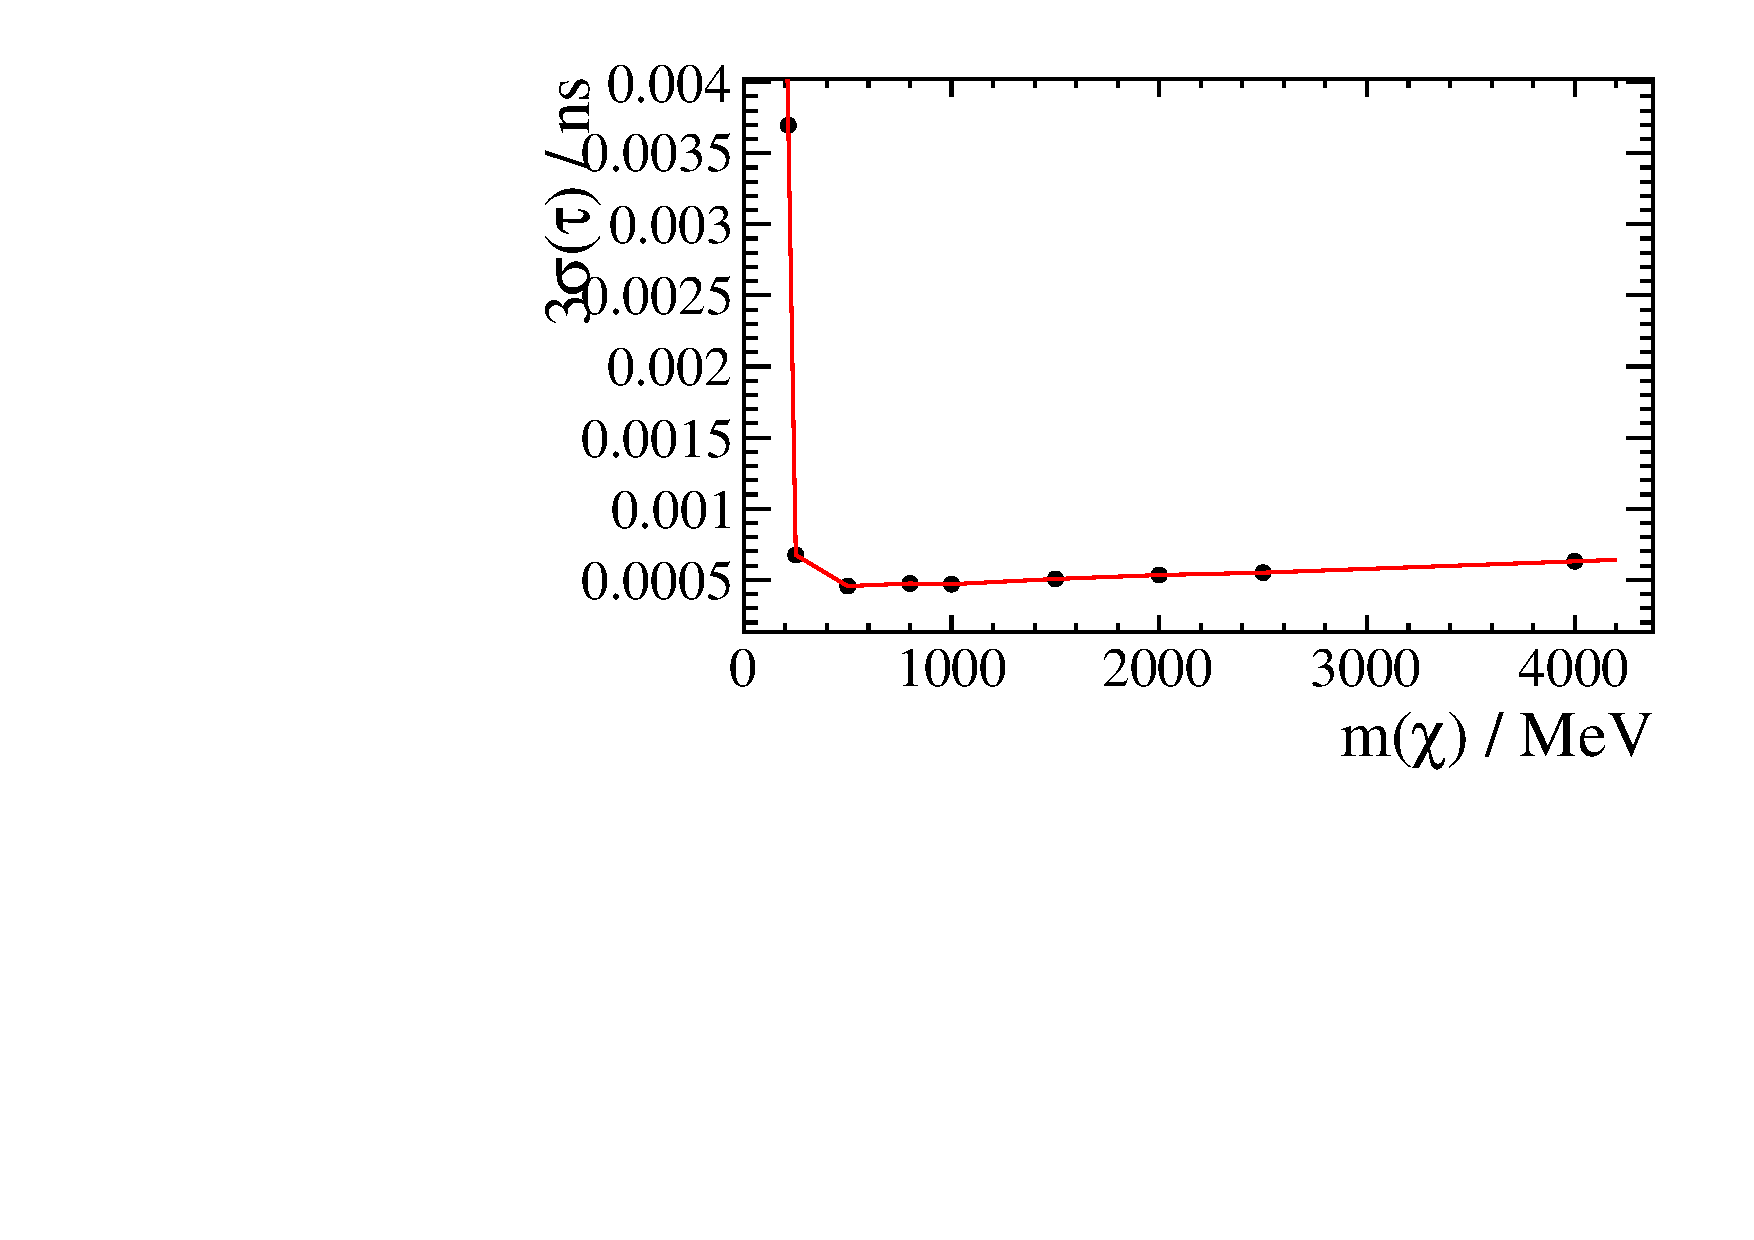
\includegraphics[width=0.48\textwidth]{spline_taures_upper}
    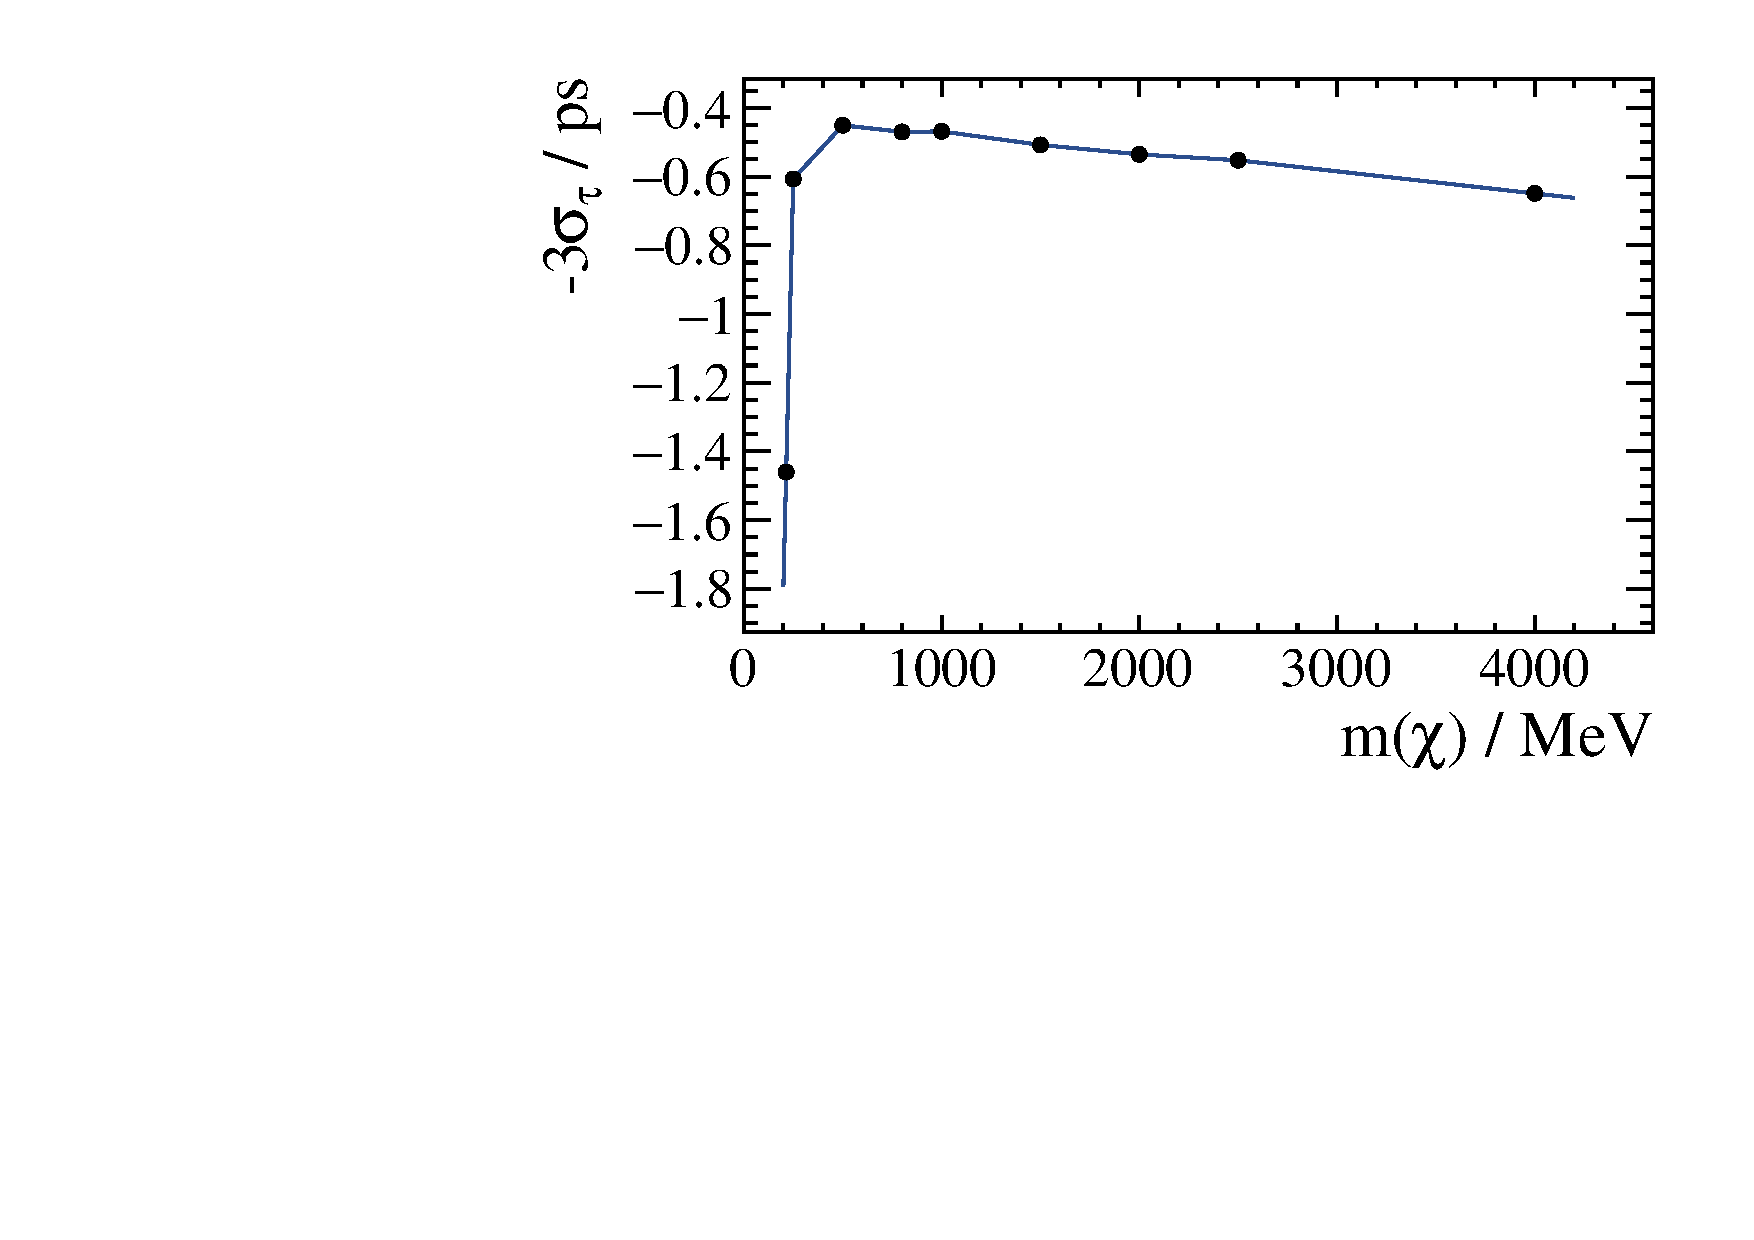
\includegraphics[width=0.48\textwidth]{spline_taures_lower}\\
    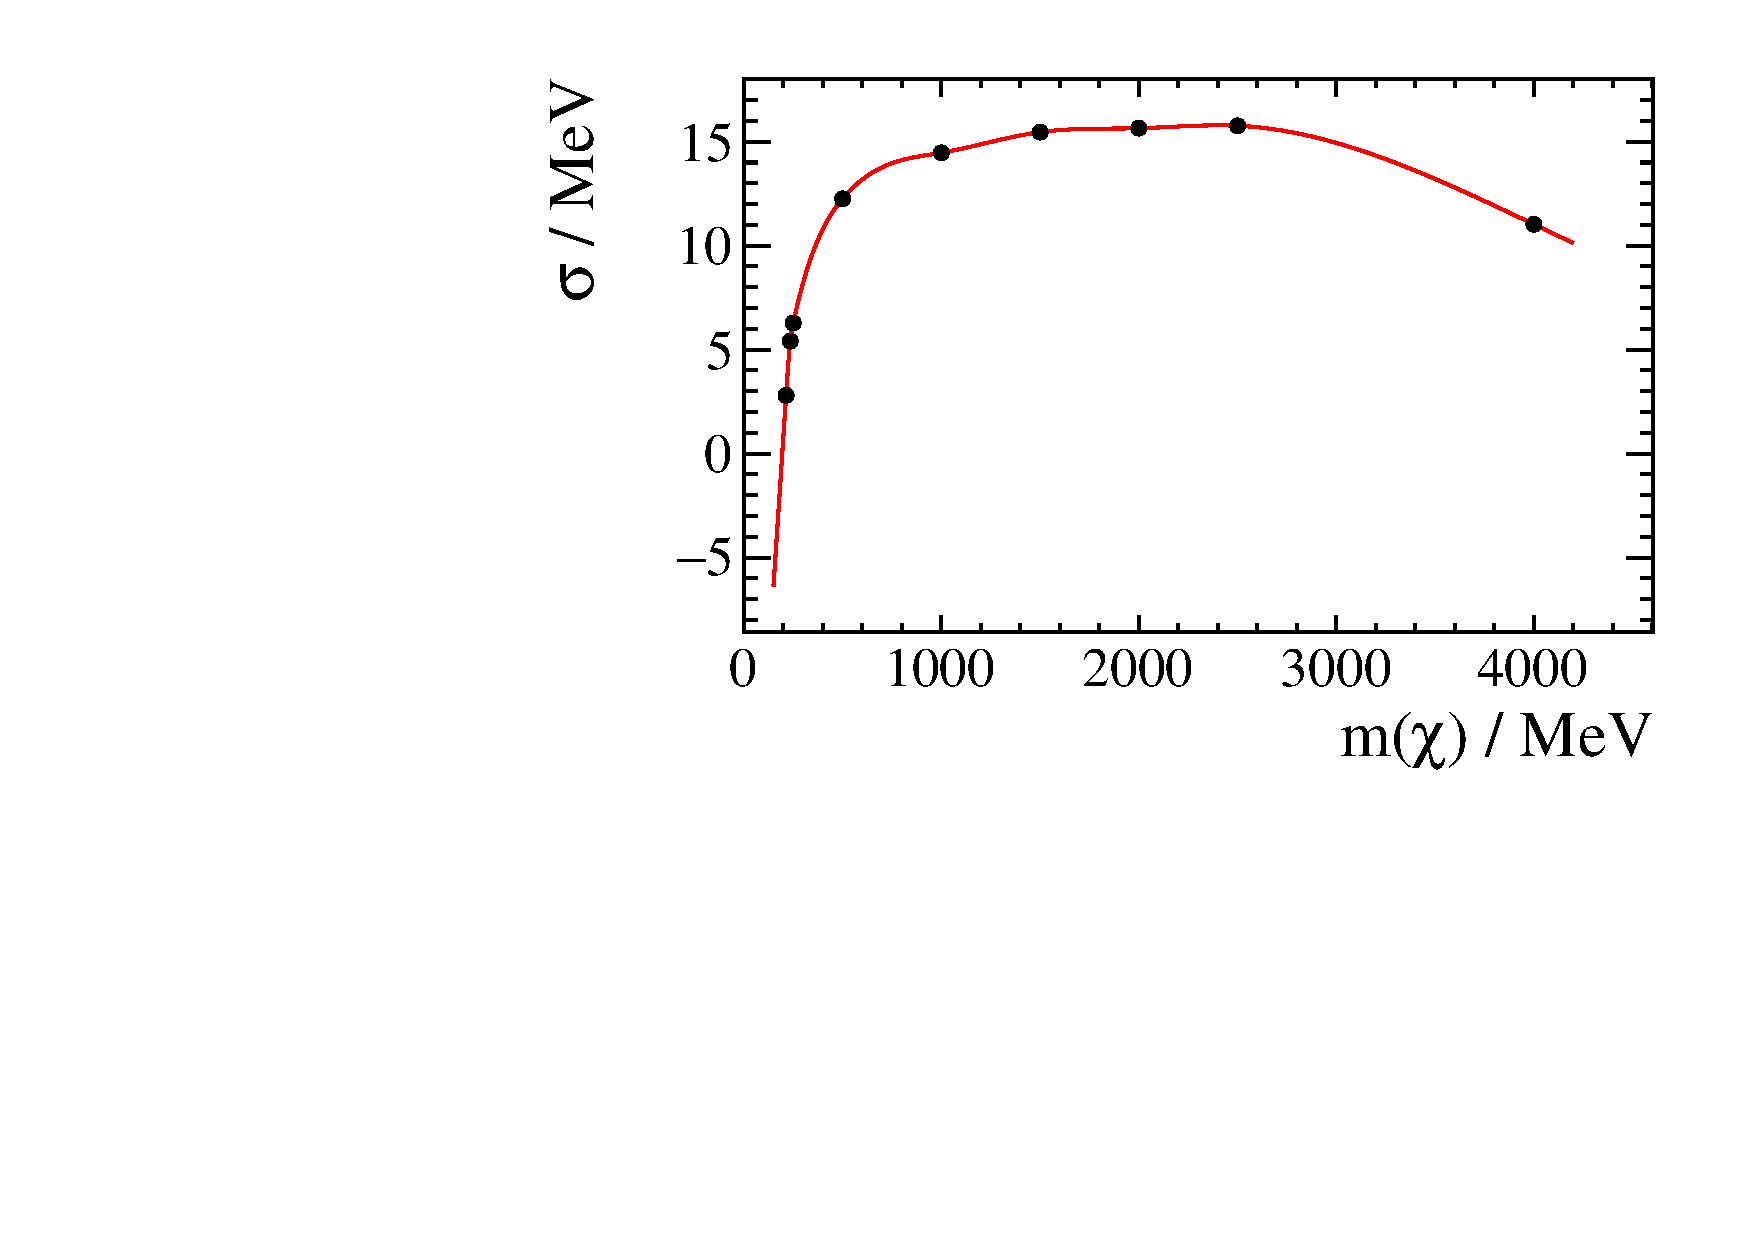
\includegraphics[width=0.48\textwidth]{spline_mass_sig}
    \caption{
      Resolutions for the lifetime of a particle as a function of mass in the
      (upper left) positive and
      (upper right) negative directions at the $3\,\sigma$ levets, used to
      define prompt and displaced regions.
      (bottom) shows the $1\,\sigma$ mass resolution as a function of
      mass.
      The black points are from fitted values and the red lines show spline interpolation.
    }
    \label{fig:eff:res}
  \end{center}
\end{figure}




\subsection{Mass resolution of the \db candidate}
The dimuon mass resolution varies as a function of $m_\mumu$.
The resolution for each simulated sample is found by fitting the mass spectrum to a
double Gaussian function.
The width of a distribution defines the resolution for a given mass, and spline interpolation is
again used to obtain the resolution for all $m_\mumu$.
Figure~\ref{fig:massres} shows the individual fits, while \Fig{fig:eff:spline:mass} shows
the mass resolution as a function of mass.


\begin{figure}
  \begin{center}
    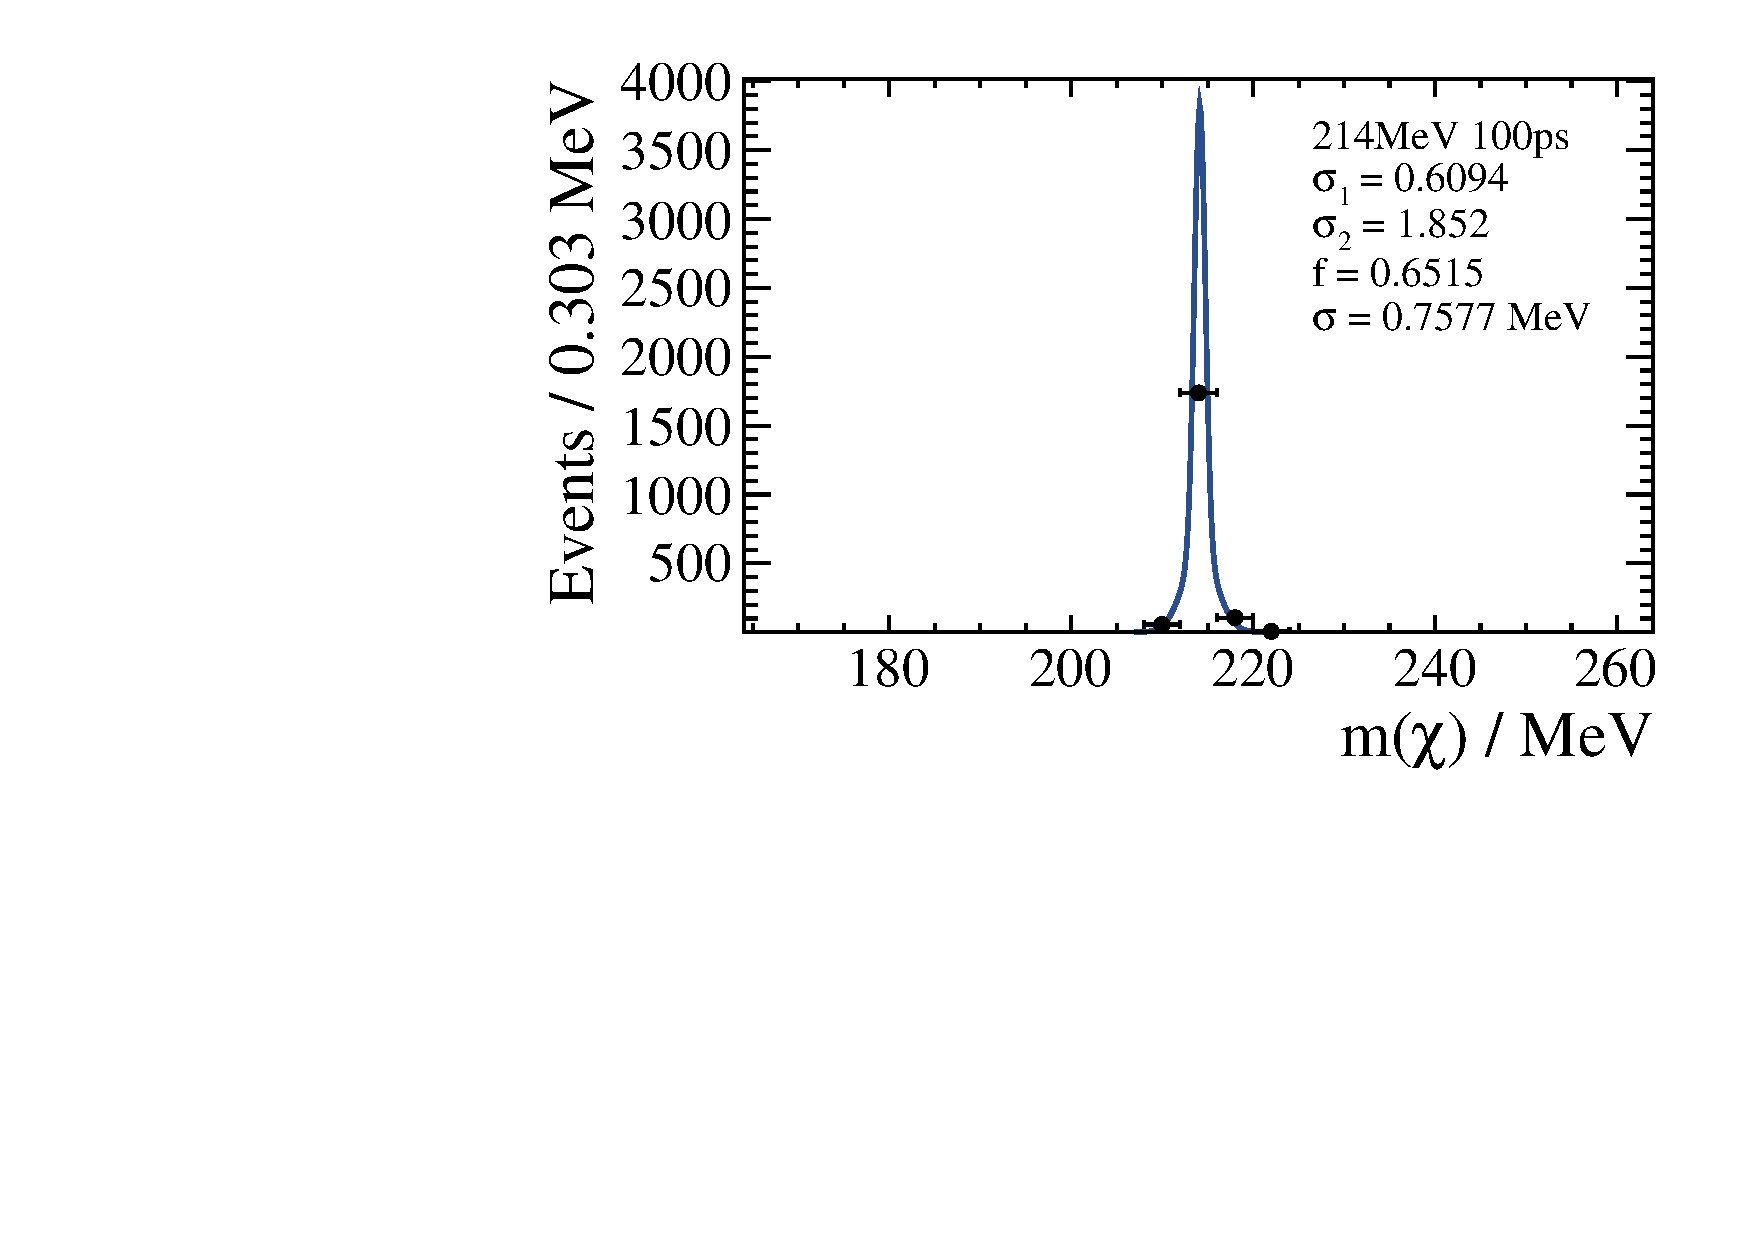
\includegraphics[width=0.42\textwidth]{anaResMass_214_100}
    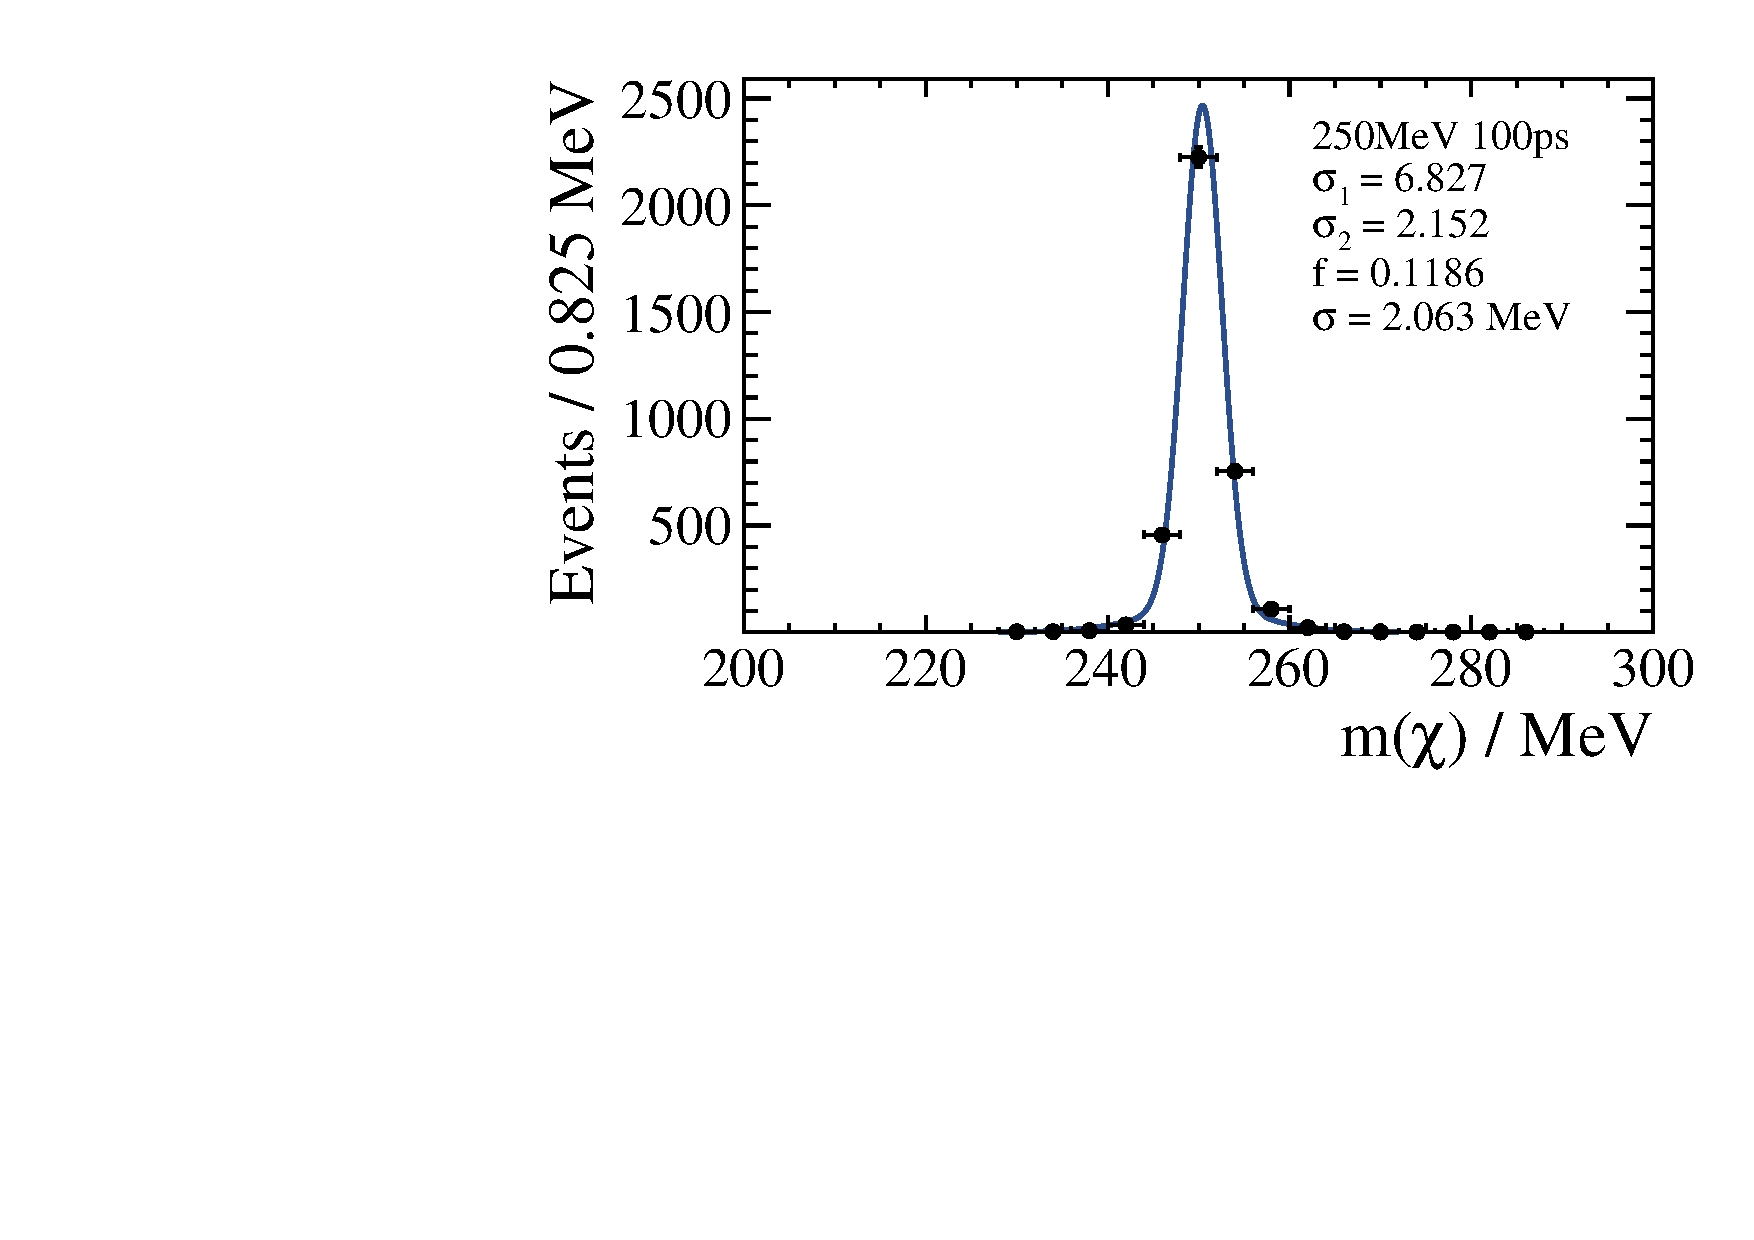
\includegraphics[width=0.42\textwidth]{anaResMass_250_100}
    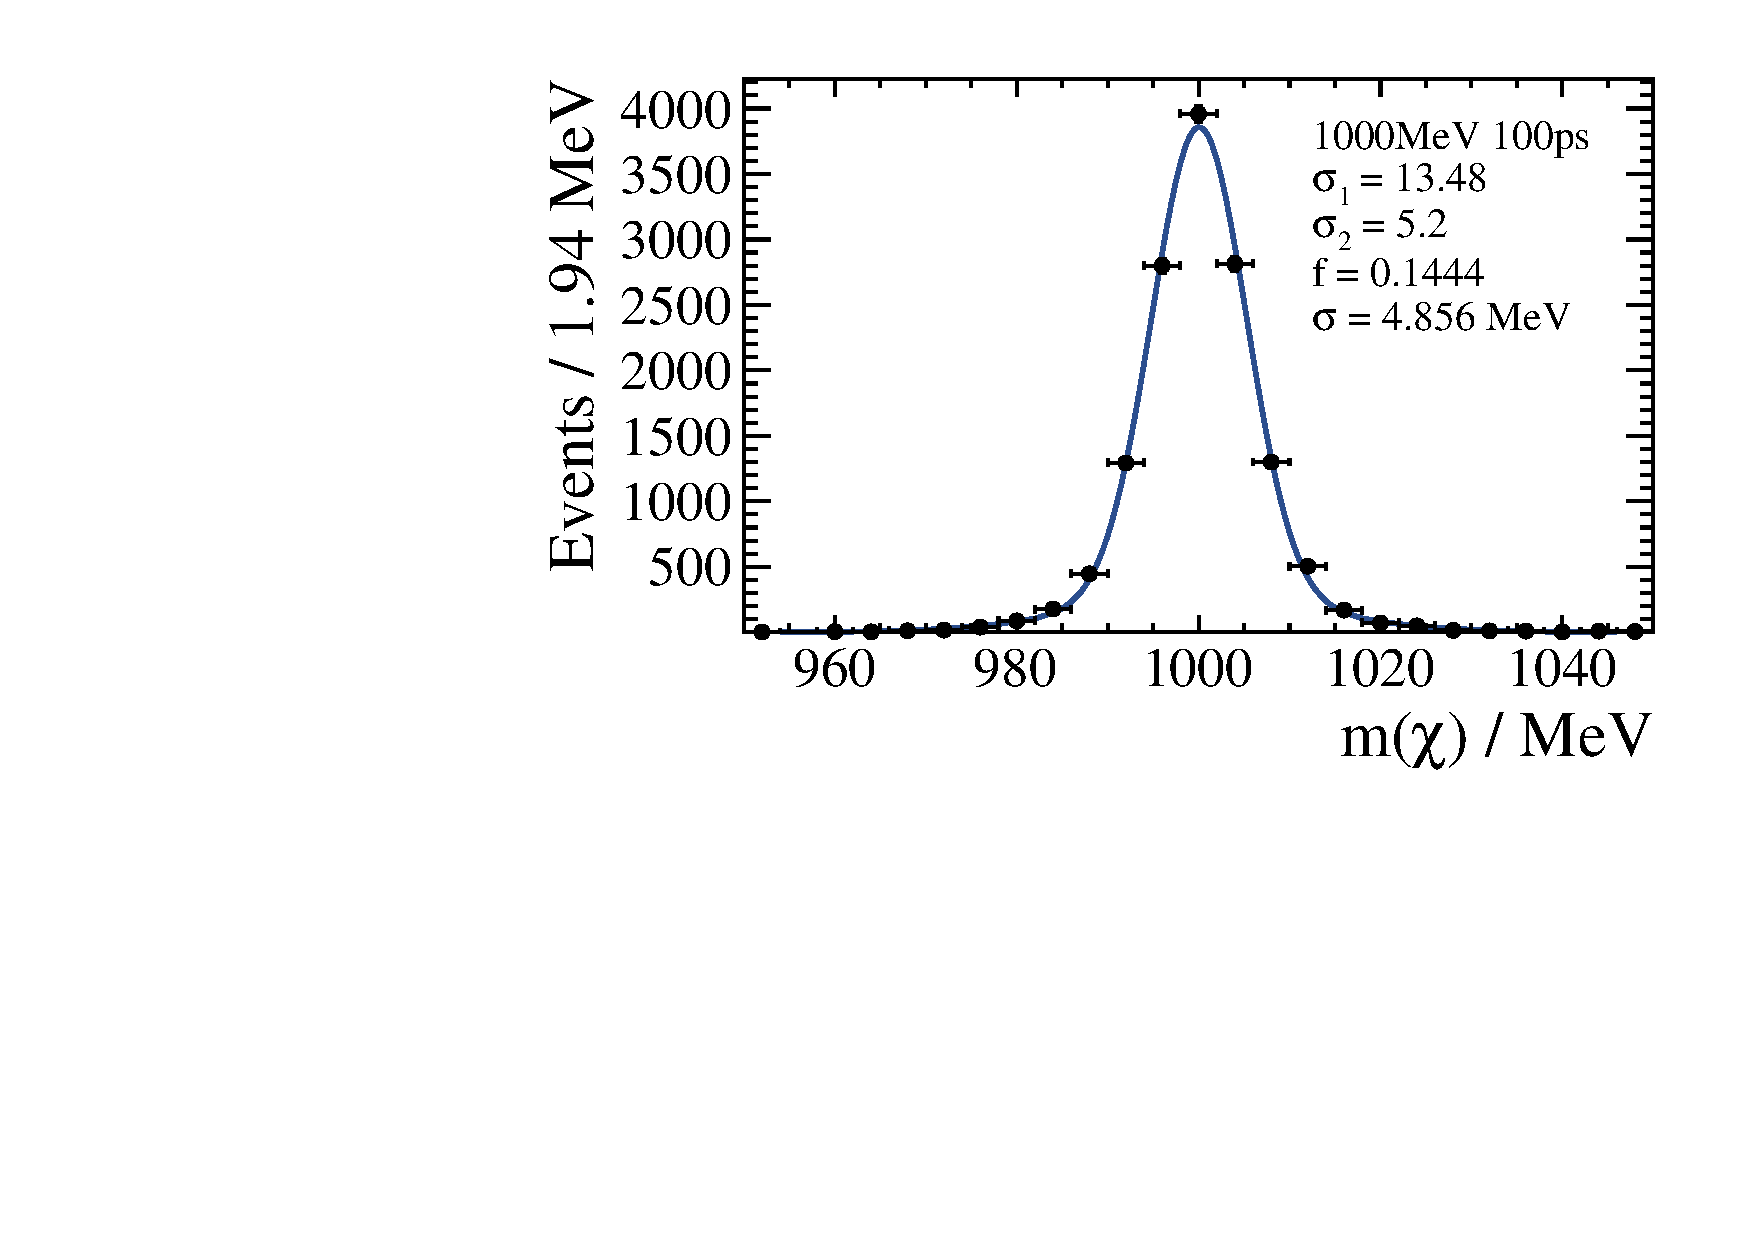
\includegraphics[width=0.42\textwidth]{anaResMass_1000_100}
    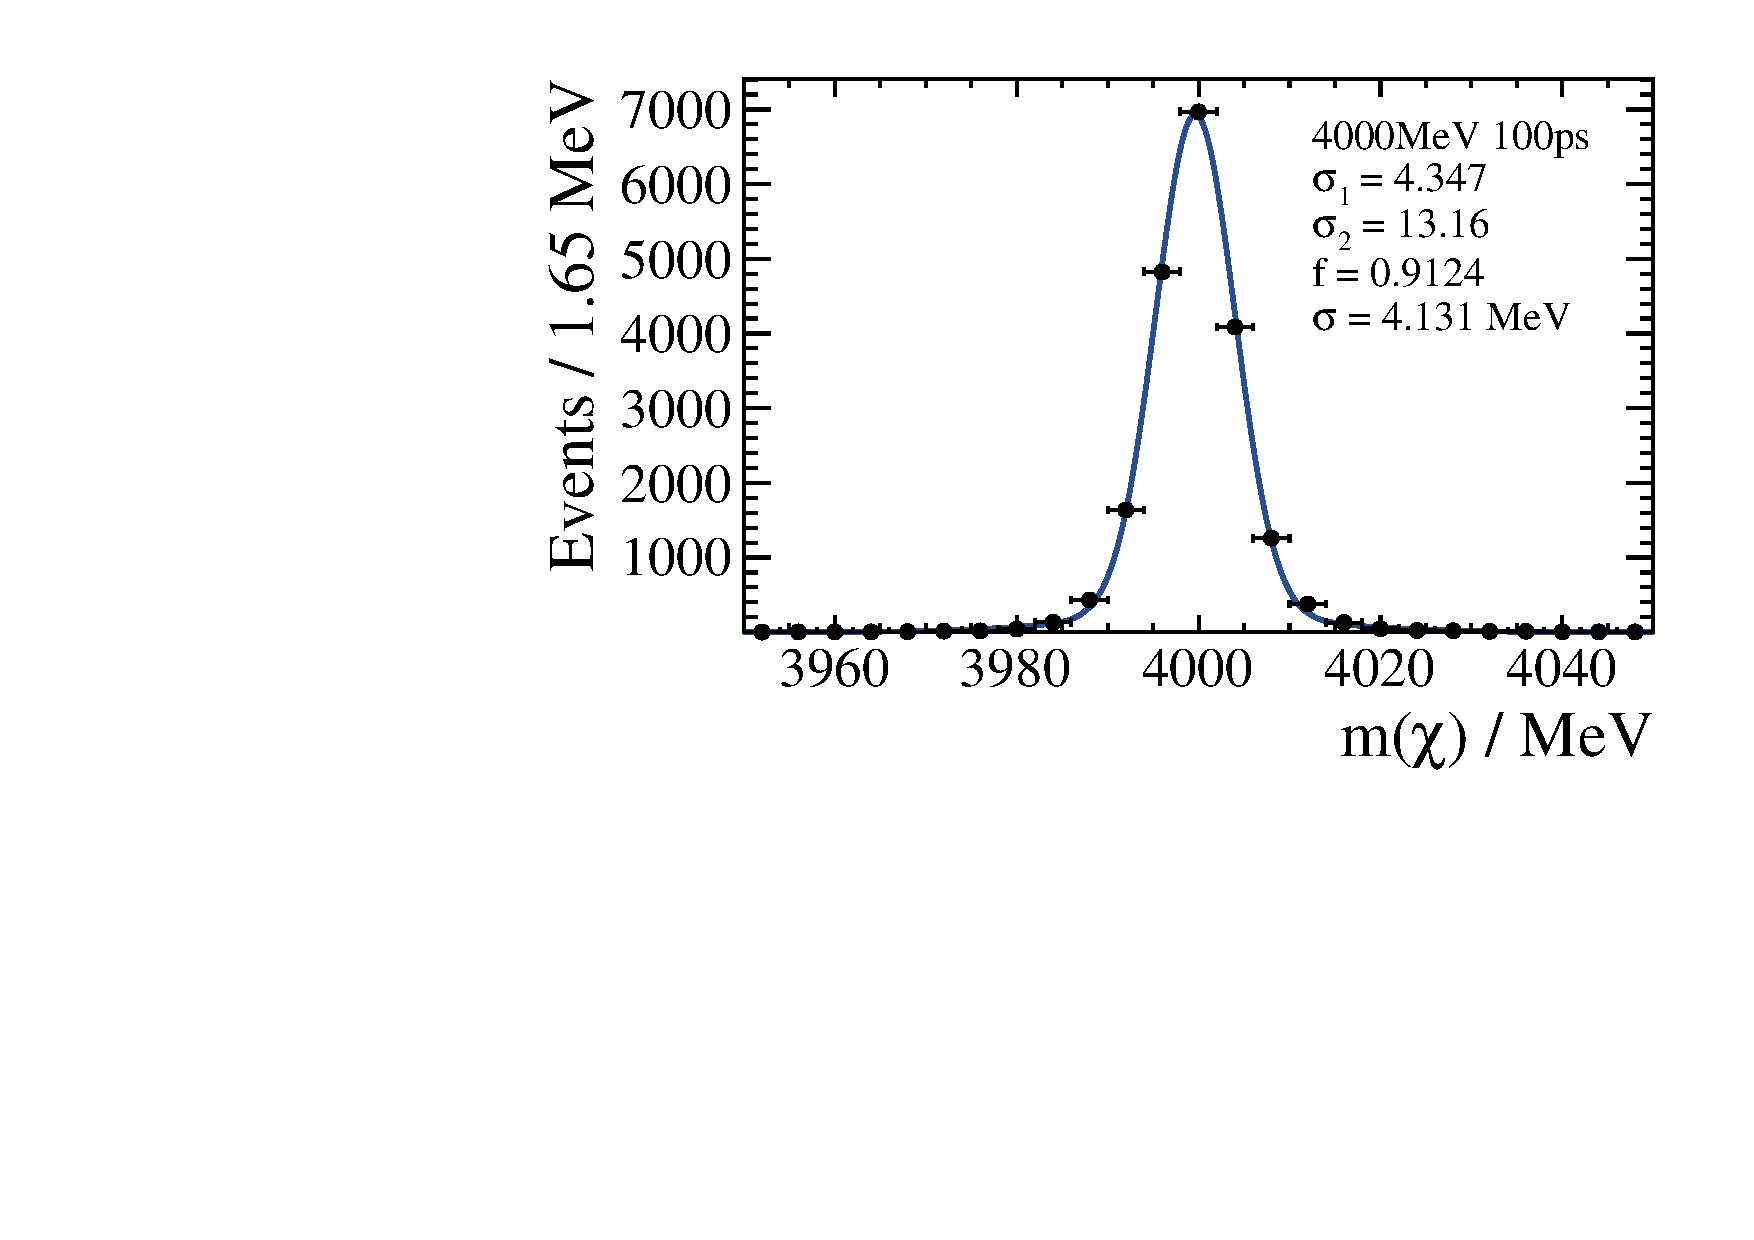
\includegraphics[width=0.42\textwidth]{anaResMass_4000_100}
  \end{center}
  \caption{
    Mass resolution for different values of \mdb, each dataset is fit to a double Gaussian
    function.
  }
  \label{fig:massres}
\end{figure}


\subsection{Parameterizing the efficiency of the \db selection}
The shape of the lifetime efficiency distribution varies with mass.
At each simulated mass point, the lifetime distribution was parameterized with a simple function,
\begin{equation}
  \mathcal{T}(\tau) = f\mathcal{G}(\mu, \sigma) + (1-f)\exp\left(-\alpha\tau\right),
  \label{eq:eff:parameters}
\end{equation}
where the parameters depends on dimuon mass.
This parameterisation is shown fitted to the lifetime distribution of four mass points in
\Fig{fig:eff:fits}.


\begin{figure}
  \begin{center}
    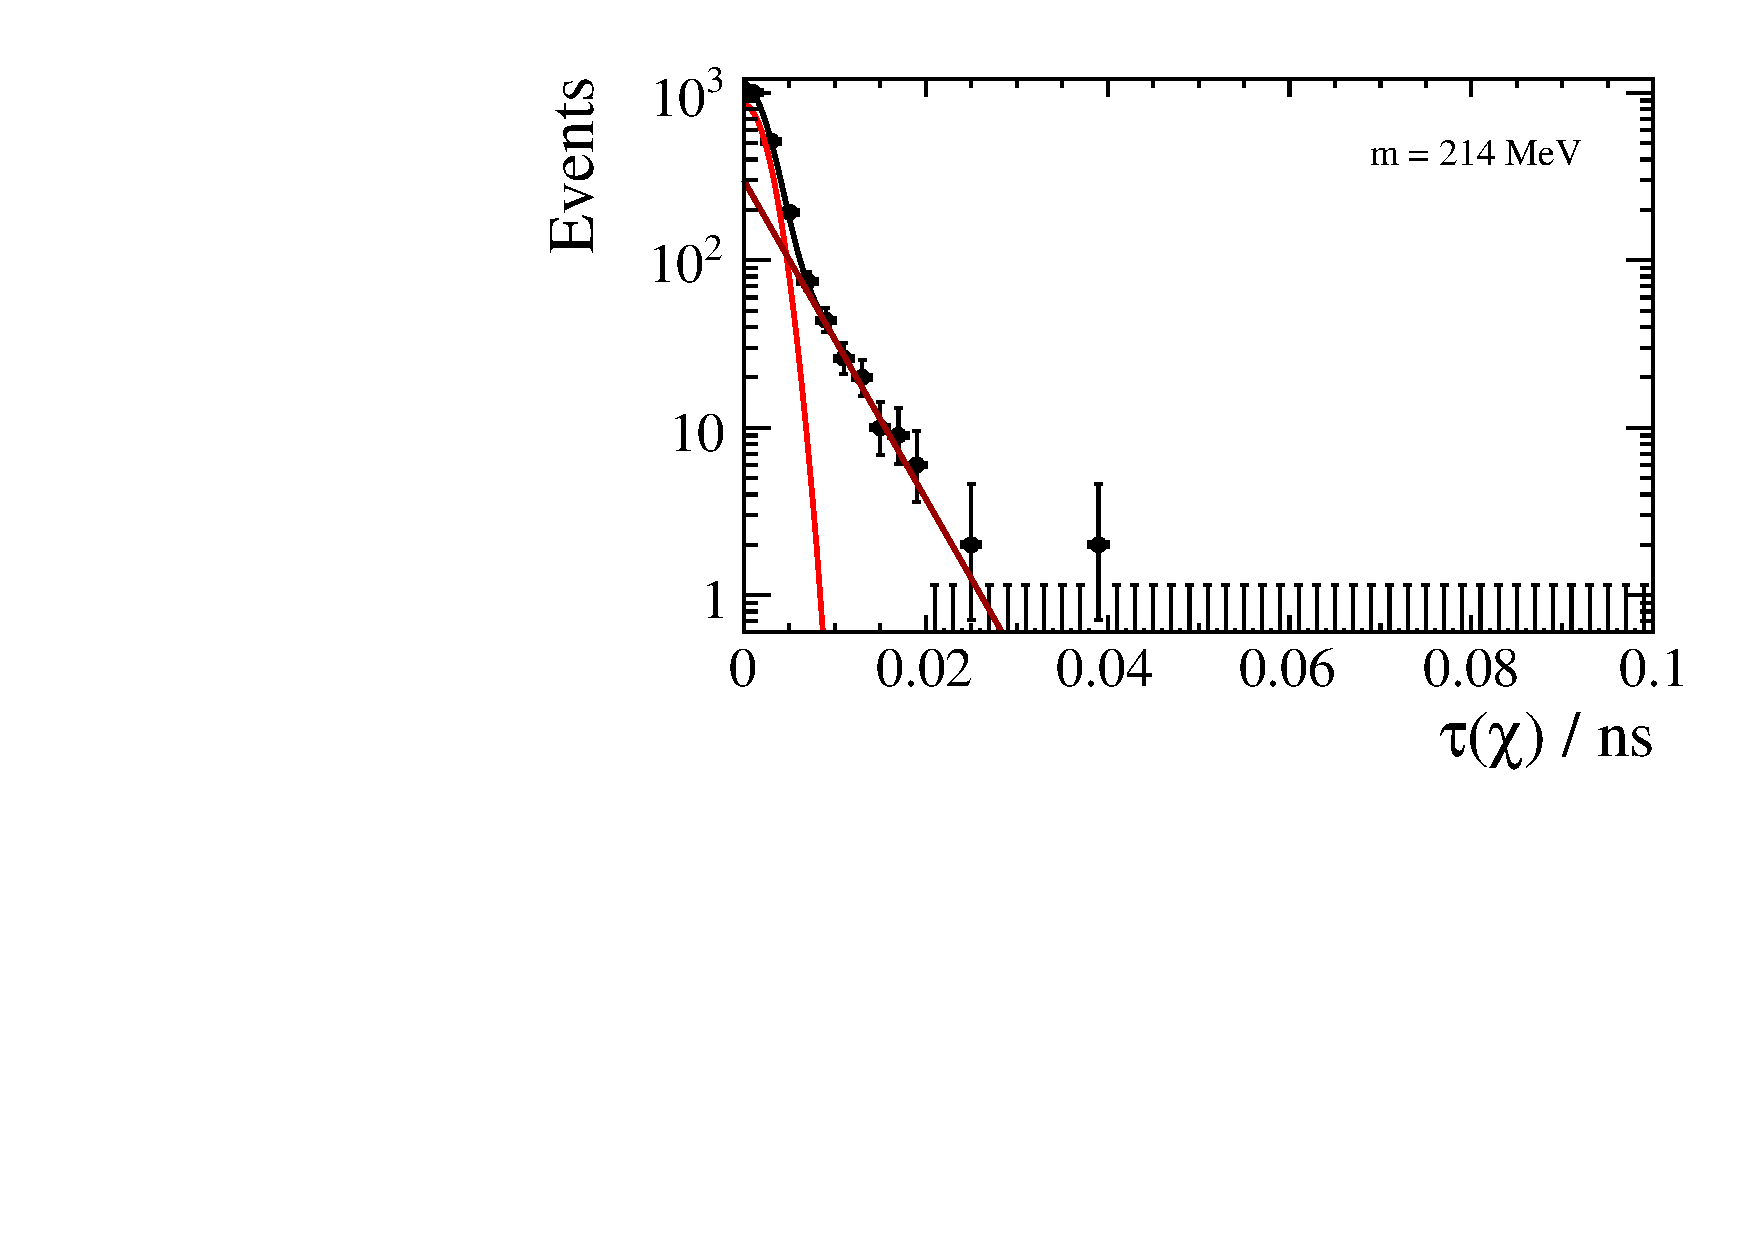
\includegraphics[width=0.48\textwidth]{anaTauEff_214}
    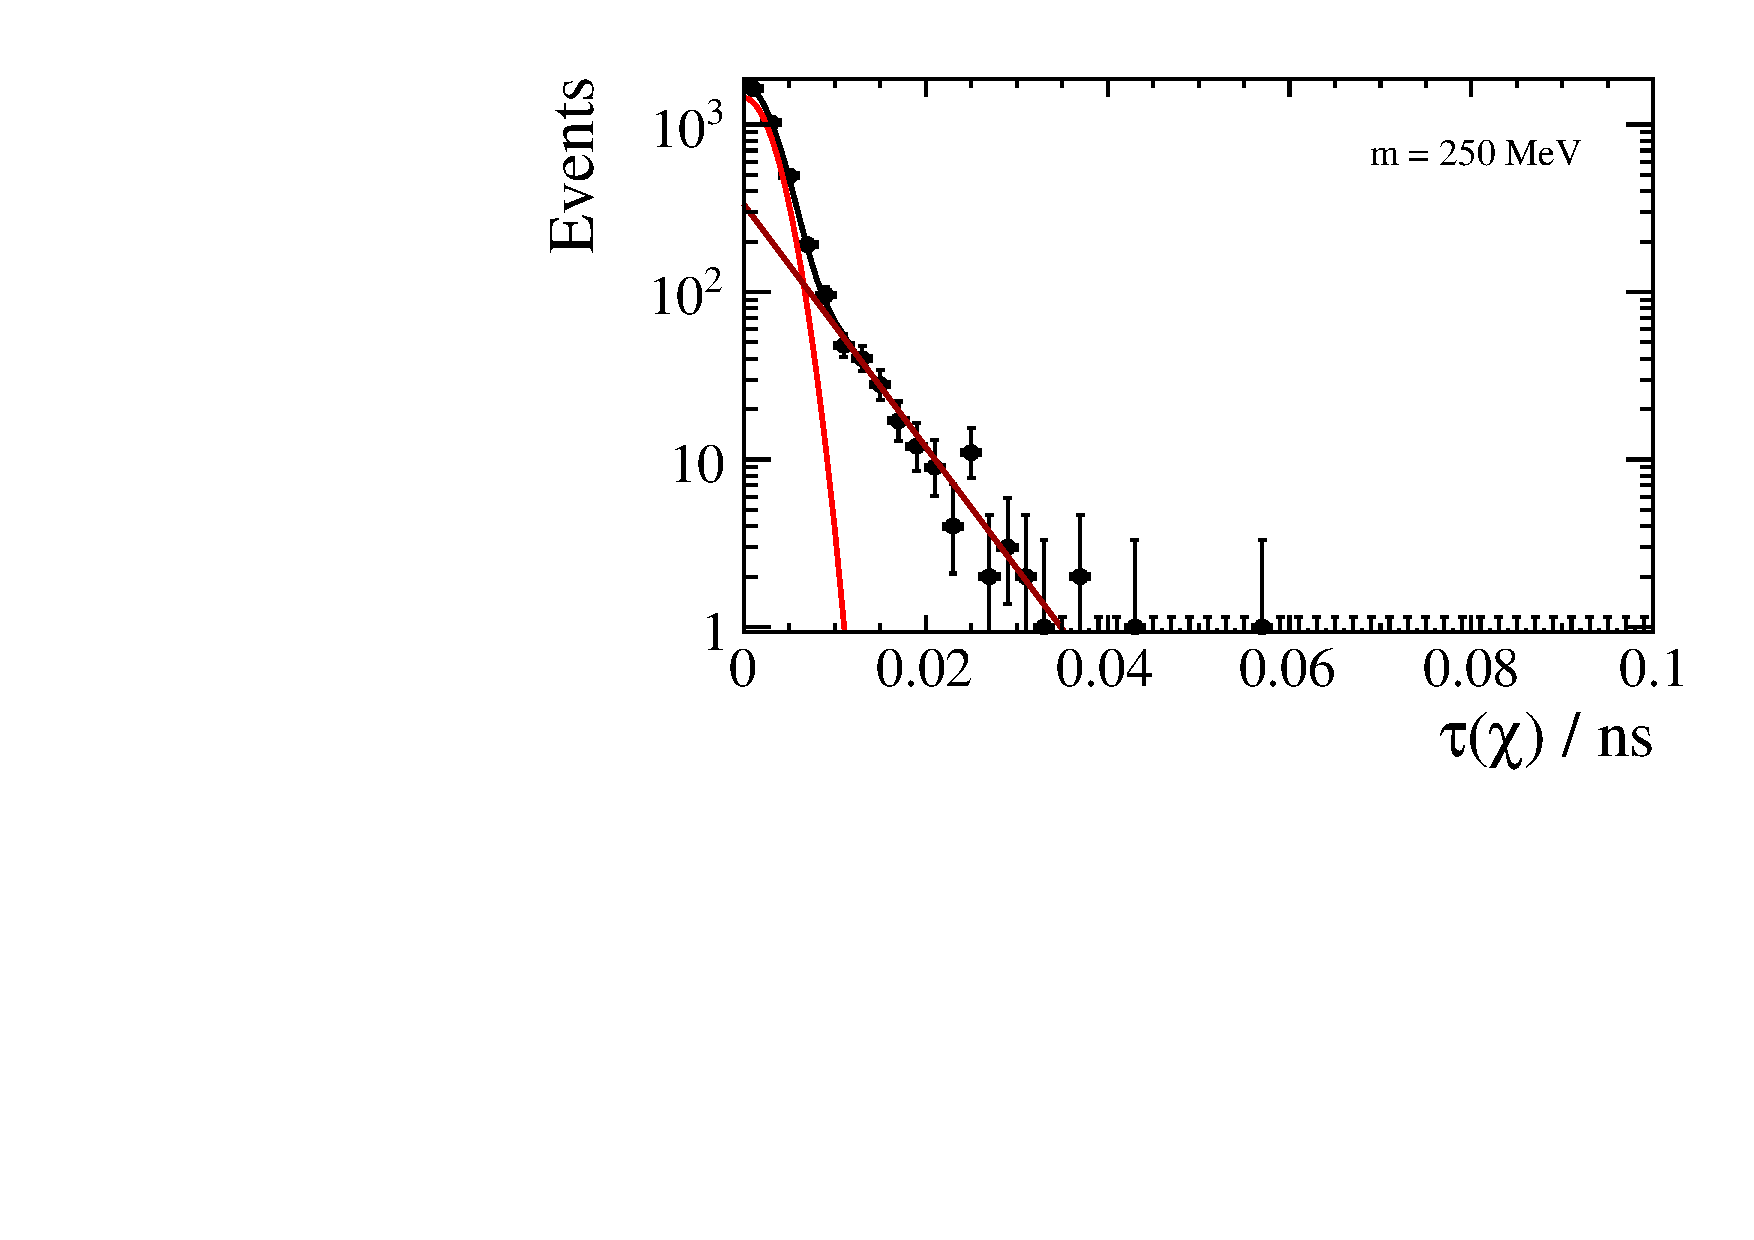
\includegraphics[width=0.48\textwidth]{anaTauEff_250}\\
    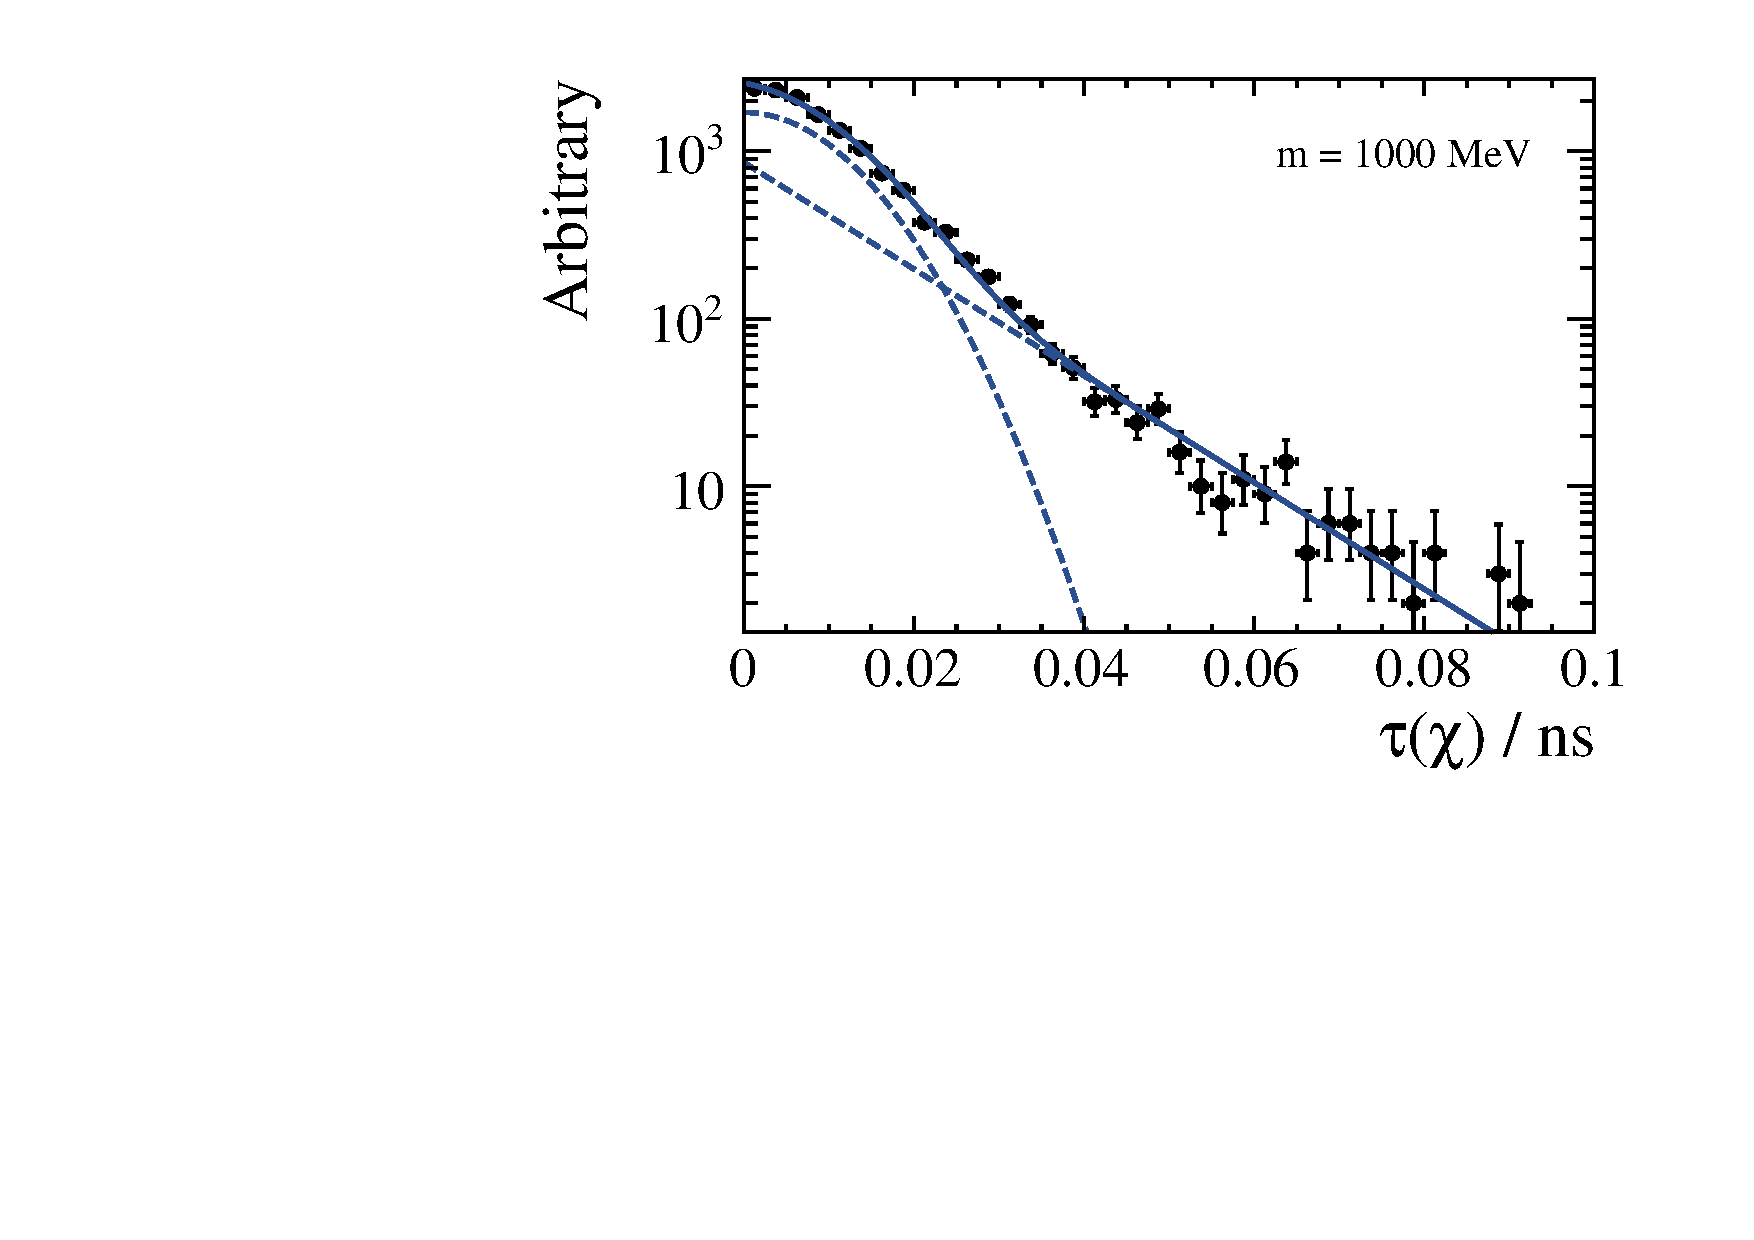
\includegraphics[width=0.48\textwidth]{anaTauEff_1000}
    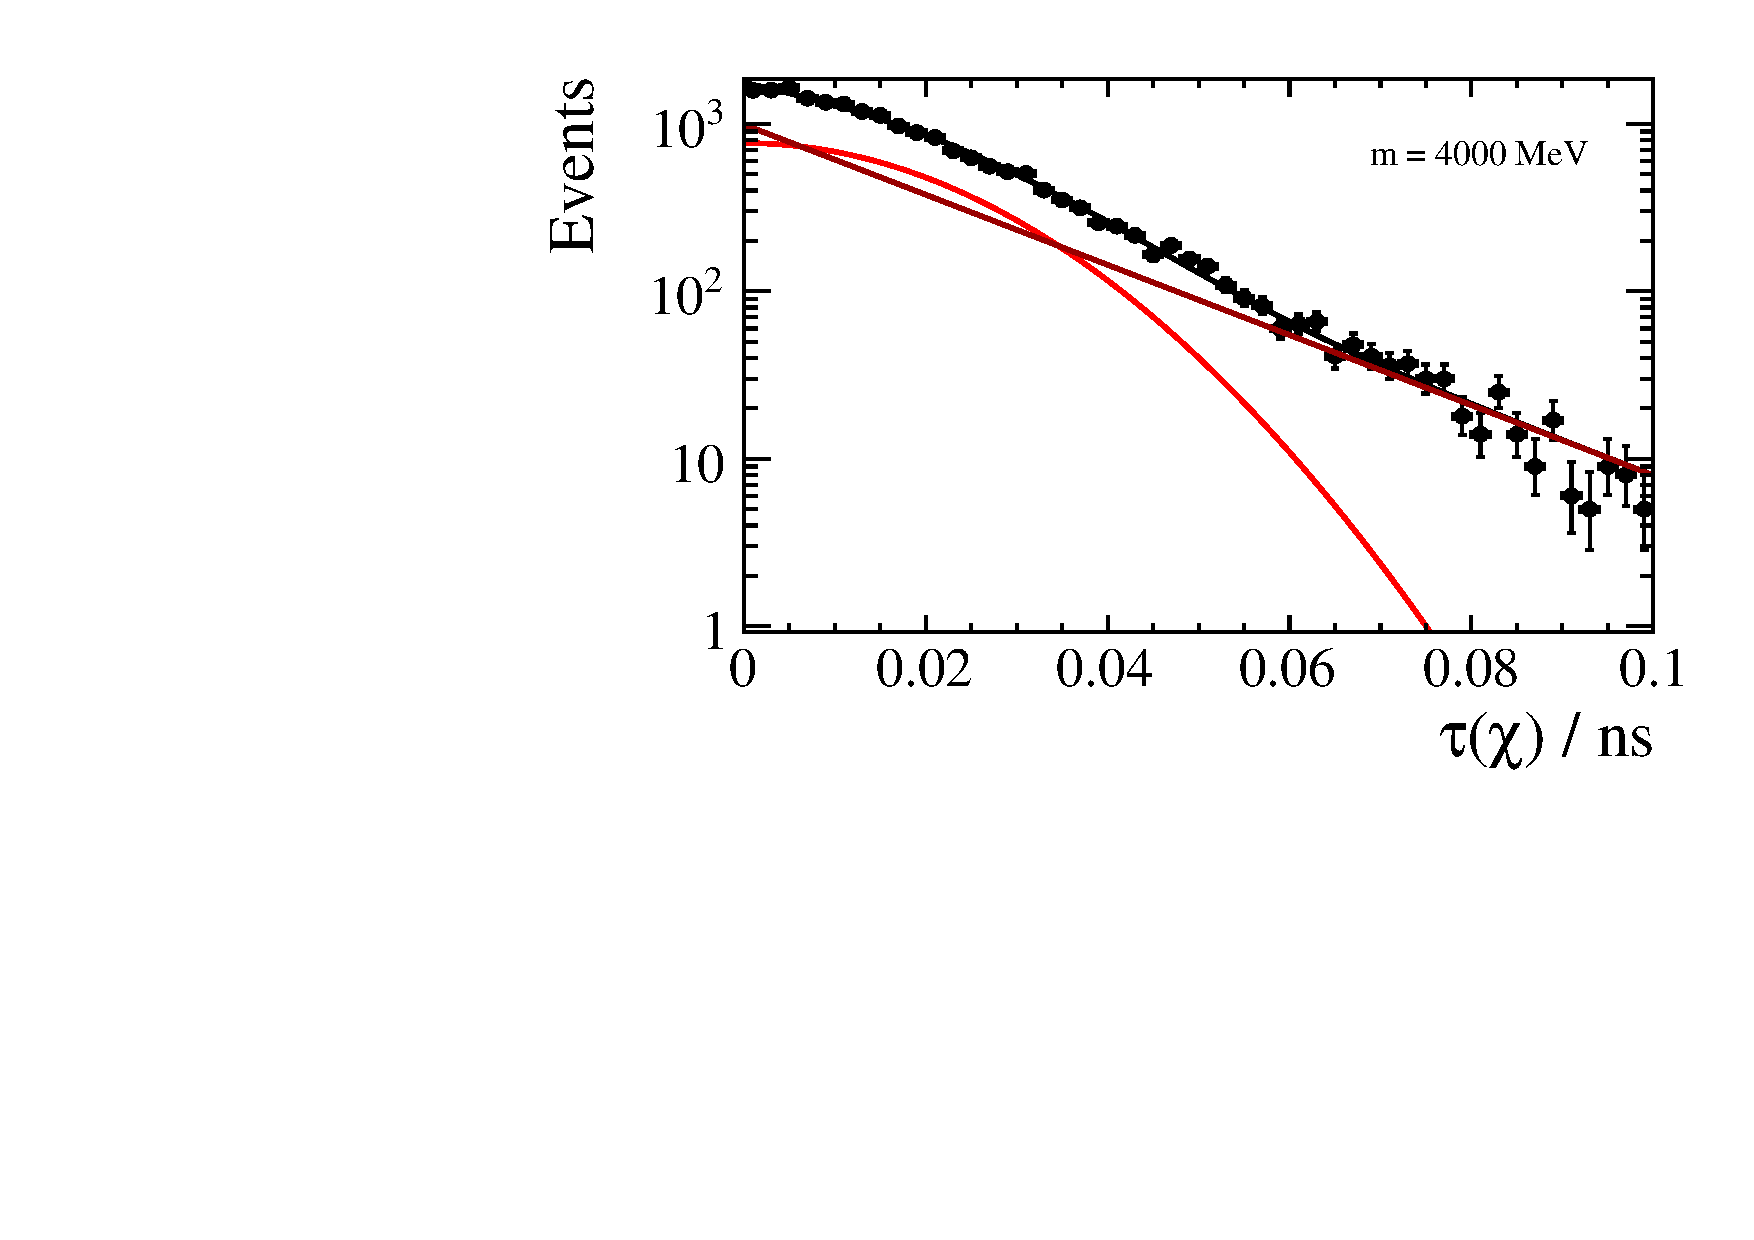
\includegraphics[width=0.48\textwidth]{anaTauEff_4000}
    \caption{\small
      Fits, using the function in Eq.~\protect\ref{eq:eff:parameters},
      to the lifetime distributions of simulated events produced with the masses:
      214, 250, 1000, and $4000\mev$ (as indicated)
      each with $\tau_\db=100\ps$.
      The black points are the simulated events, and the black line is the total fit, with light
      and dark red lines showing the Gaussian and exponential components, respectively.
    }
    \label{fig:eff:fits}
  \end{center}
\end{figure}


Samples with different masses are fit with the results for each parameter plotted against dimuon
mass in \Fig{fig:eff:spline}.
Extrapolation to different masses is done using spline interpolation, as shown in
\Fig{fig:eff:spline}.
The value of $f$ has large errors, and has little effect on the total shape.
A cubic spline models this very poorly because of the fluctuations at low mass, therefore linear
regression is used instead.
These splines account for all efficiencies except for the efficiency of the uBDT and the geometric
acceptance of the \lhcb detector; the uBDT and geometric acceptance are nearly the same for all
samples and so nearly cancel in the limit setting.
An example of a lifetime efficiency distribution for a given mass is shown in \Fig{fig:eff:effmap},
as is the two-dimensional projection, absolute efficiencies have not been included in this.

The efficiency map shown in \Fig{fig:res:mbvtau} was generated using simulated samples where
$\tau(\db)=100\ps$ but contains the efficiency at each $\tau$ below 100\ps.
It is then possible to obtain the efficiency for any other lifetime as follows:
\begin{equation}
  \varepsilon(\tau) =
  \frac{1}{\tau}\int\limits_0^{100\ps}
  \mathcal{T}(\tau^{\prime})
  \exp\left(-\frac{\tau^{\prime}}{\tau}\right)
  \,{\rm d}\tau^{\prime},
%  \left.\exp\left(-\frac{\tau}{x}\right)\right/
%  \exp\left(-\frac{\tau}{100\ps}\right),
\end{equation}
%where $x$ is the `target' lifetime, in ps.
The upper lifetime acceptance will be $100\ps$, this is because the efficiency for longer lifetimes
is very poor.


\begin{figure}
  \begin{center}
    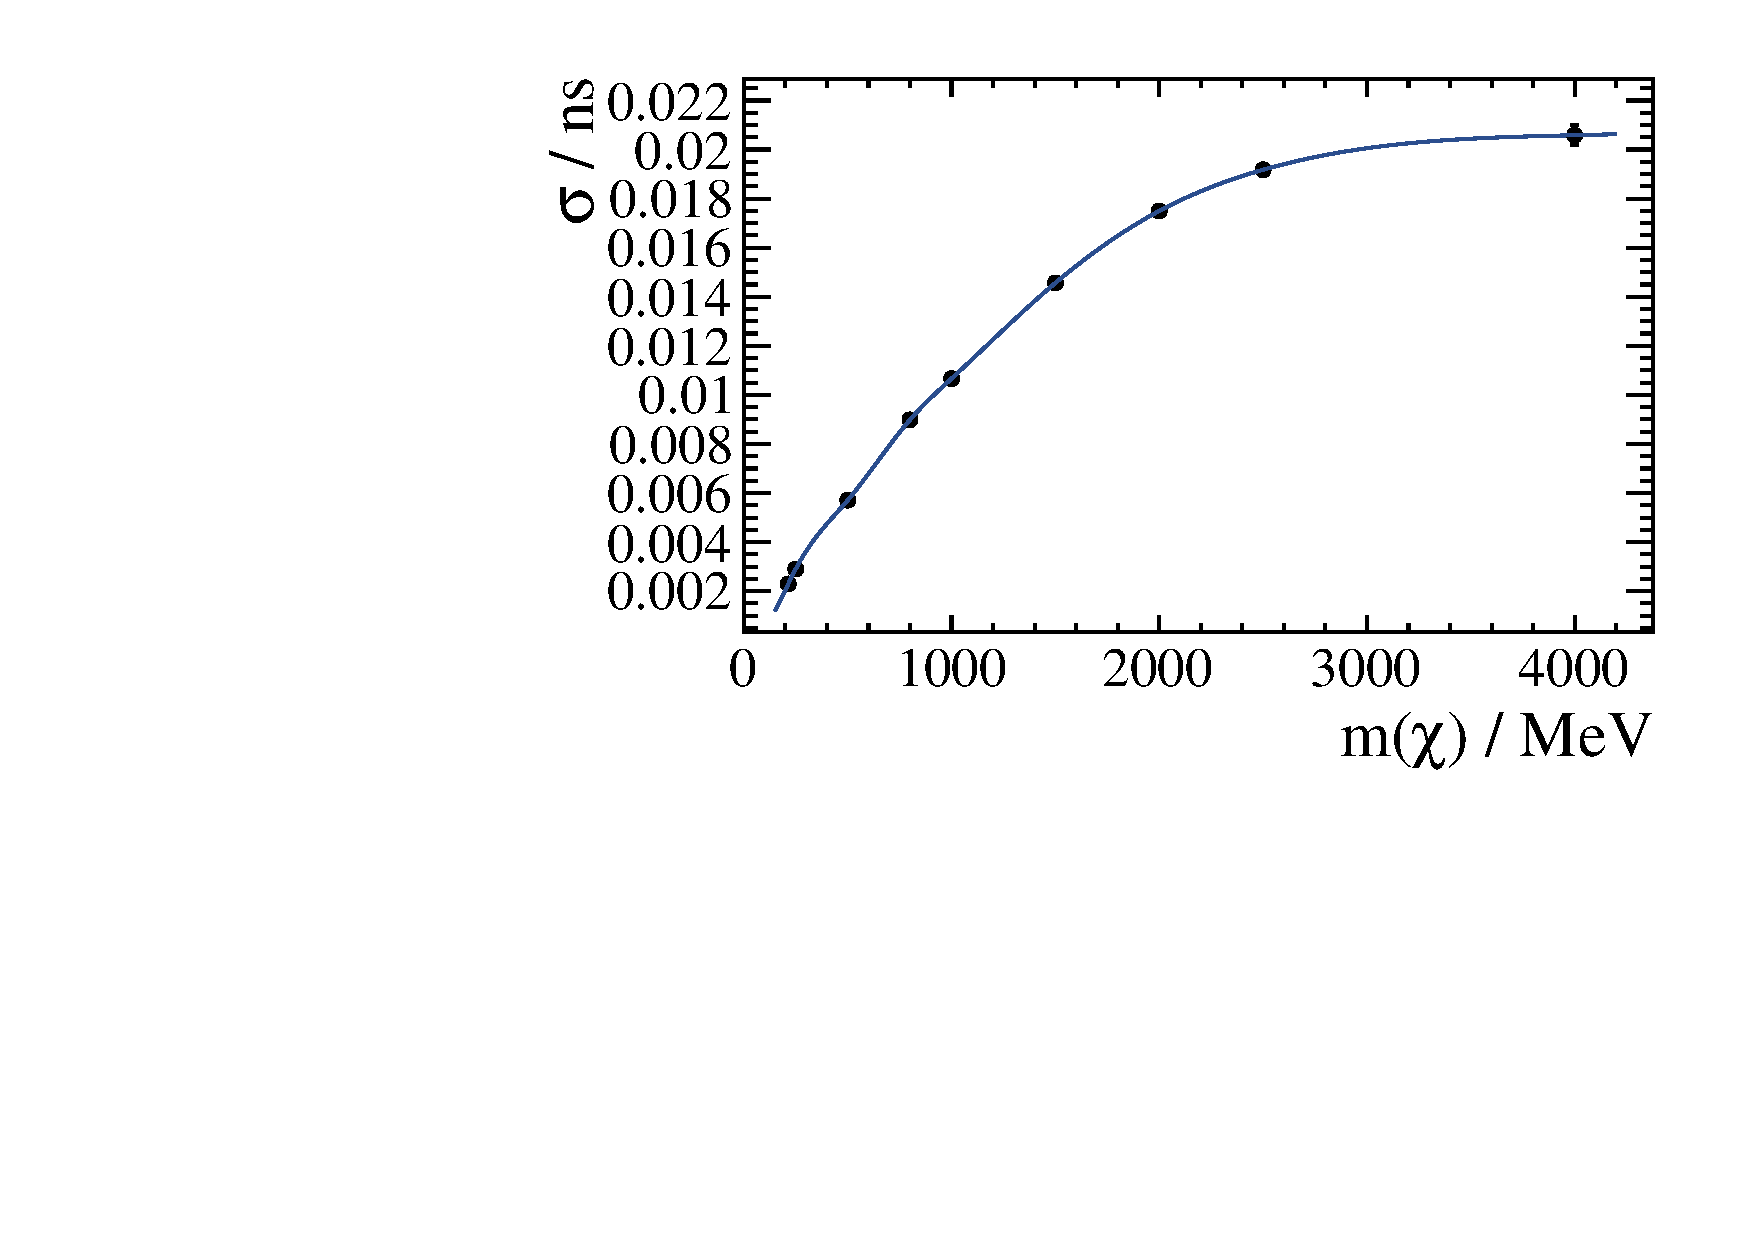
\includegraphics[width=0.48\textwidth]{spline_sigma}
    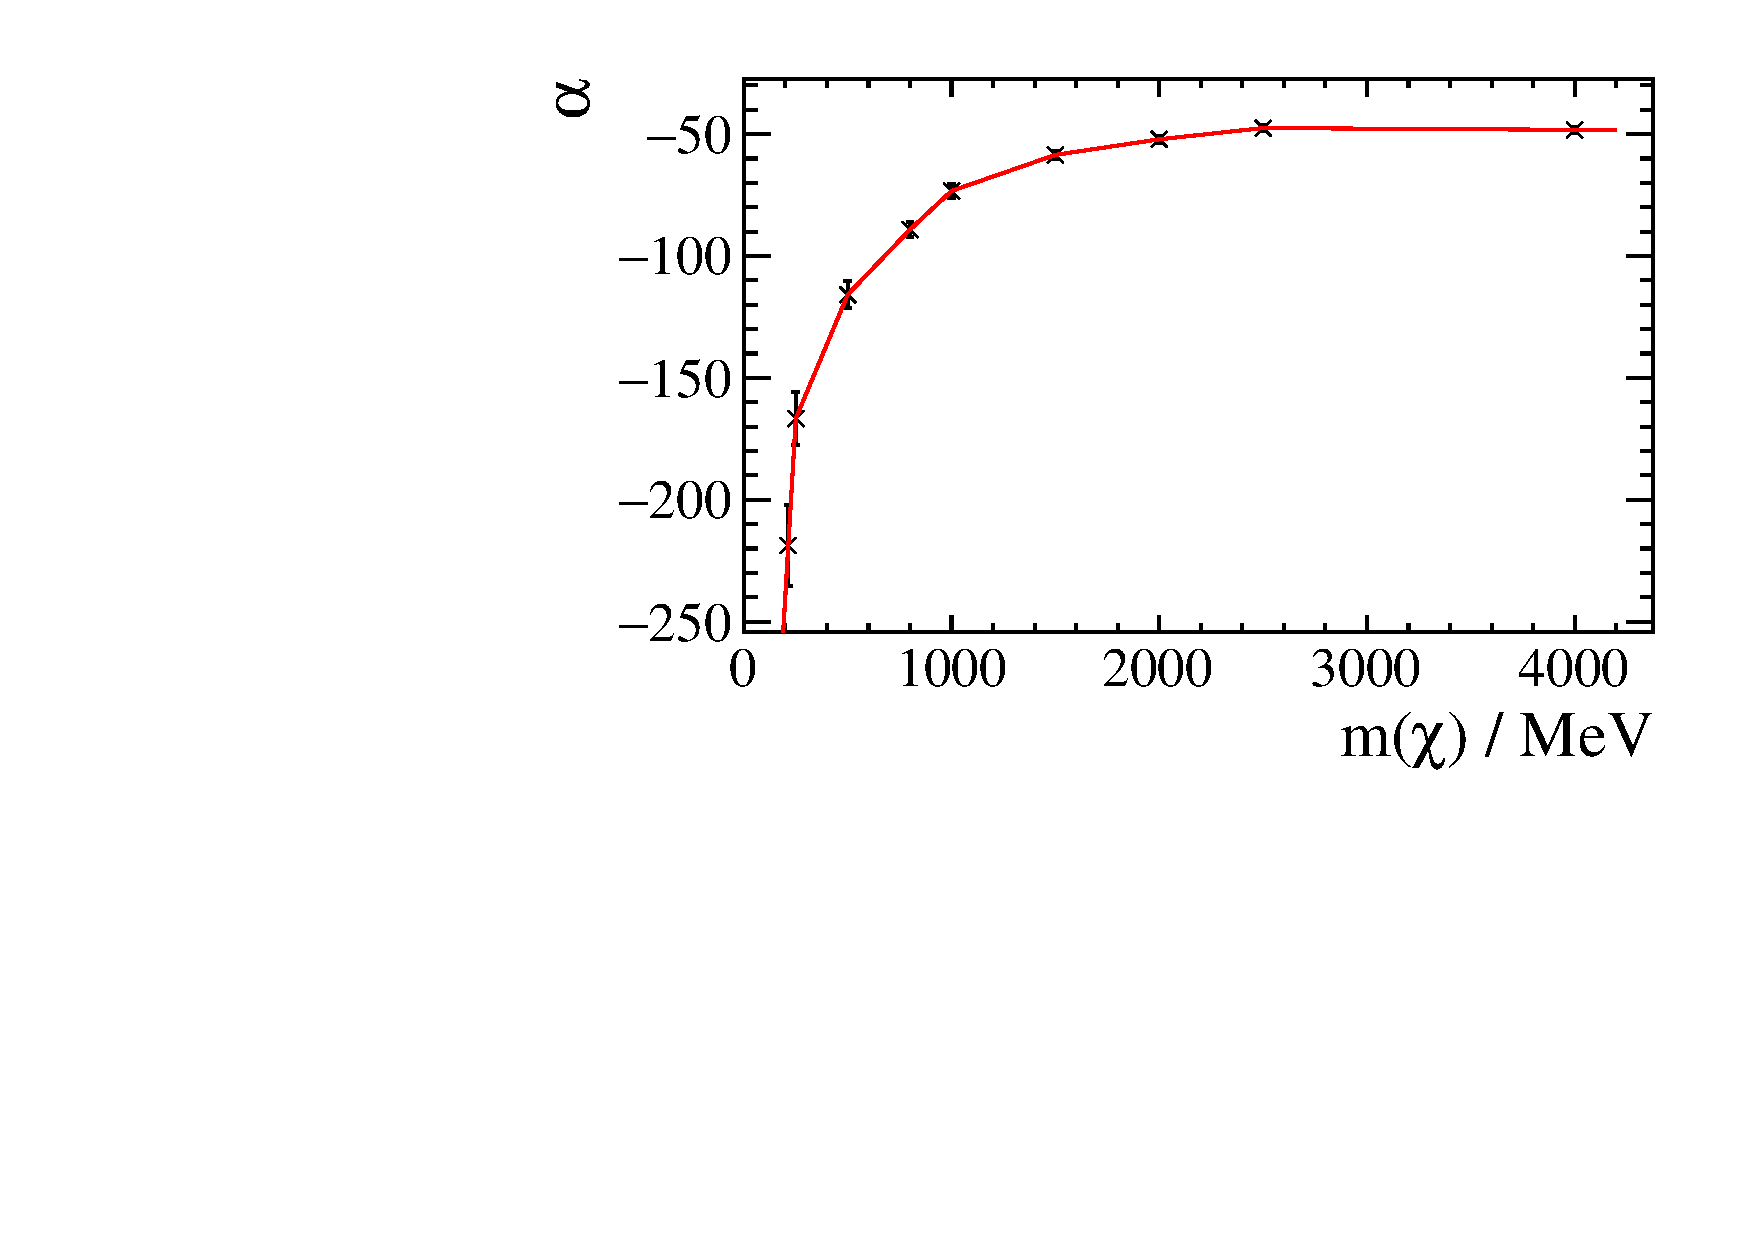
\includegraphics[width=0.48\textwidth]{spline_alpha}\\
    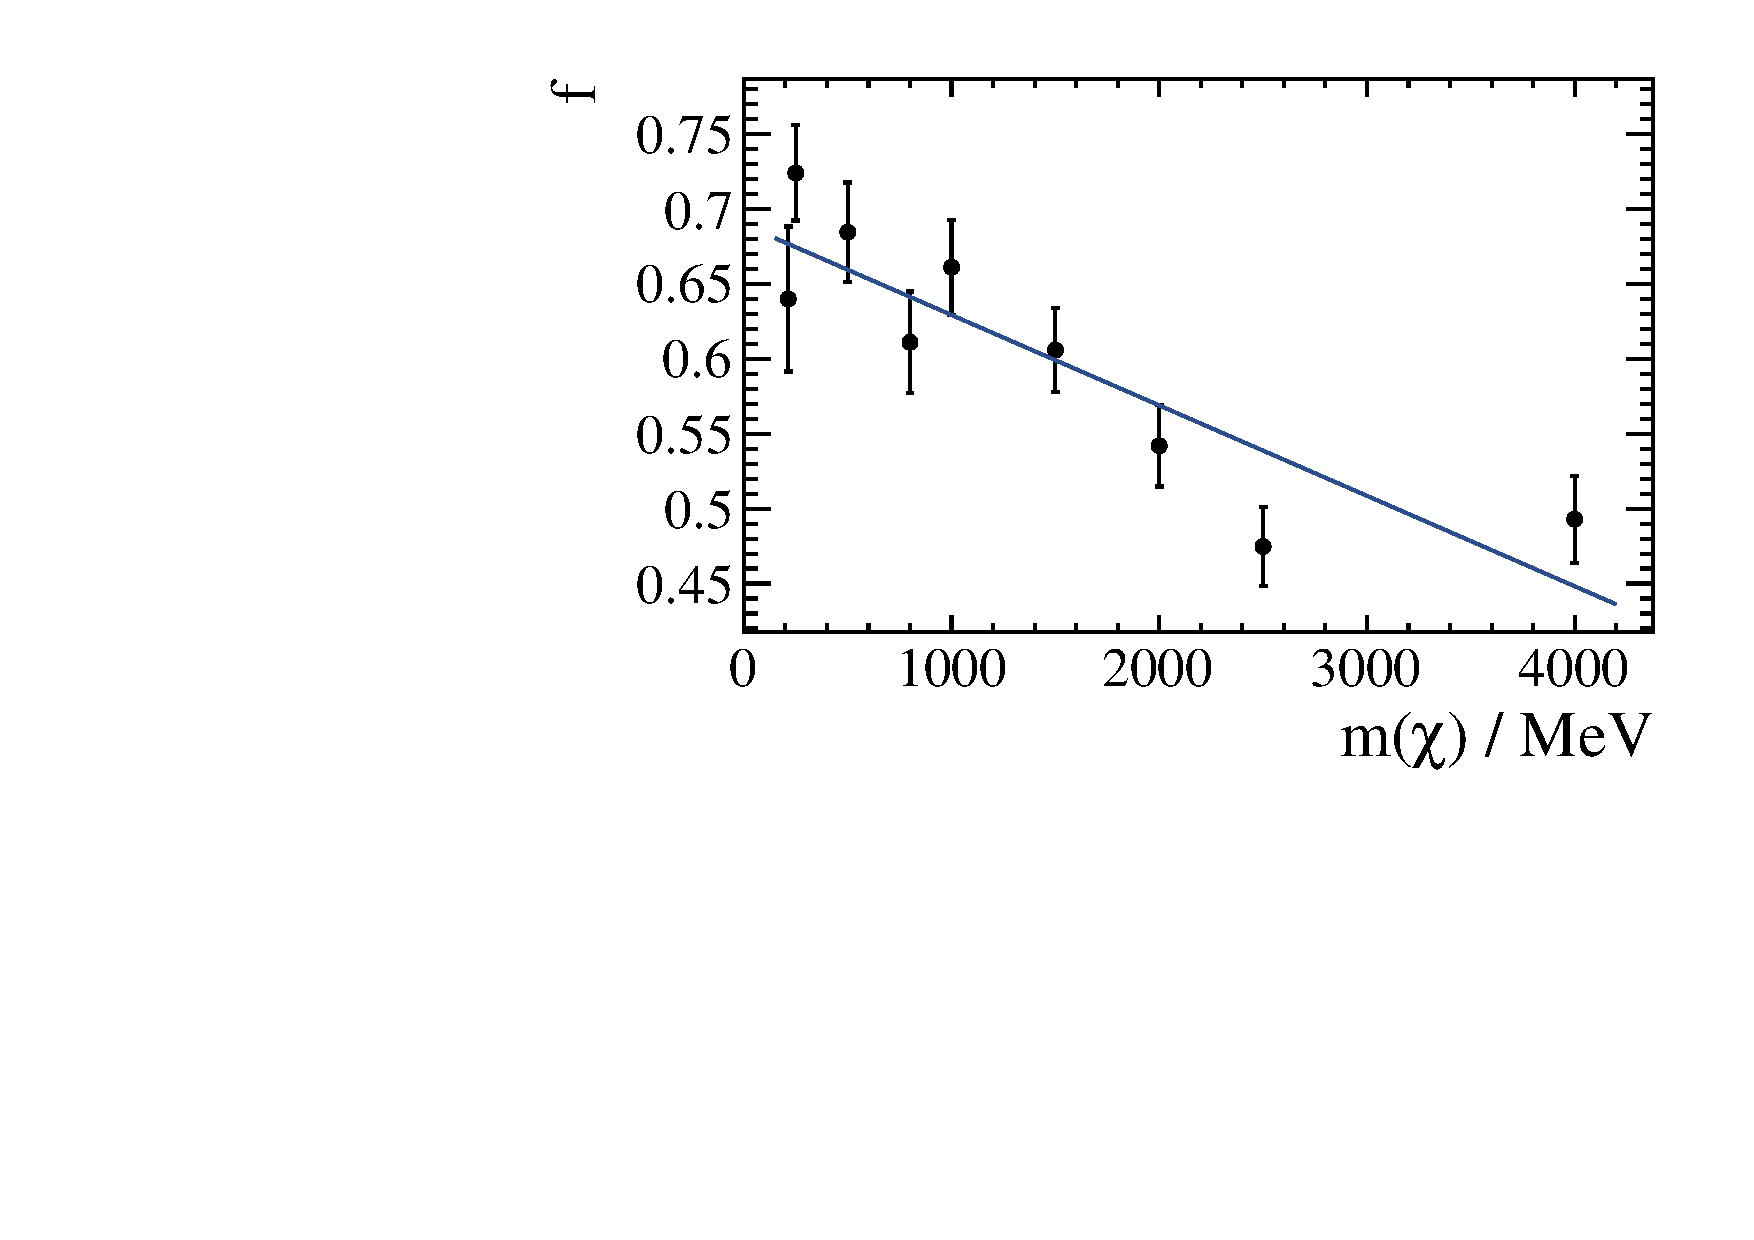
\includegraphics[width=0.48\textwidth]{spline_frac}
    \caption{
      Parameters from Eq.~\protect\ref{eq:eff:parameters} as a function of mass from
      simulated events.
      The parameters are
      (upper left) $\sigma$,
      (upper right) $\alpha$, and
      (lower) $f$.
      Splines are used to parameterize each shape, except for the parameter $f$, where a
      linear fit is used.
    }
    \label{fig:eff:spline}
  \end{center}
\end{figure}

\begin{figure}
  \begin{center}
    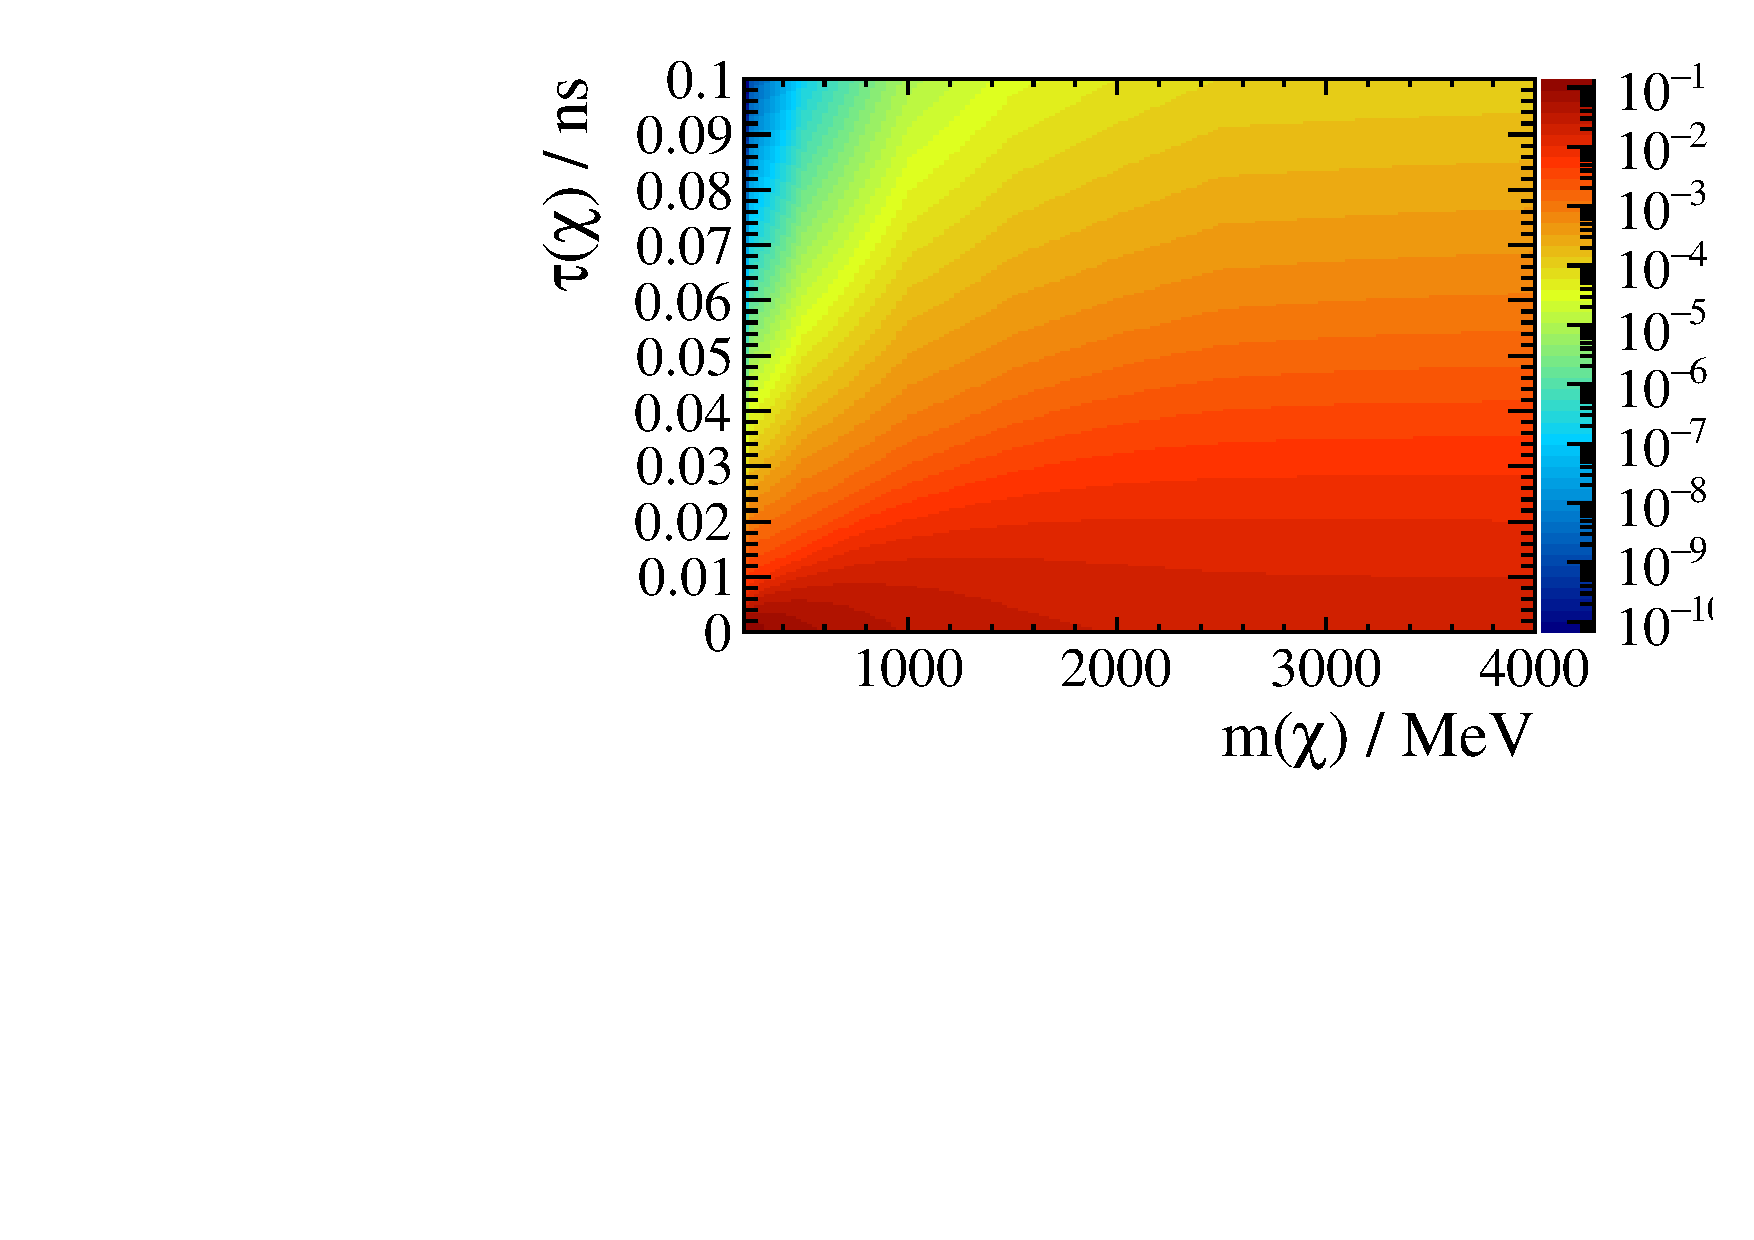
\includegraphics[width=0.48\textwidth]{spline_2d}
    \caption{
      Using the parameters in Fig.~\ref{fig:eff:spline} and Eq.~\protect\ref{eq:eff:parameters} the
      lifetime distributions are formed for the full two-dimensional projection.
      Absolute efficiencies are not folded in here.
    }
    \label{fig:eff:effmap}
  \end{center}
\end{figure}



\subsection{Efficiency studies using \decay{\Bd}{\jpsi\Kstarz}}










